\PassOptionsToPackage{unicode=true}{hyperref} % options for packages loaded elsewhere
\PassOptionsToPackage{hyphens}{url}
%
\documentclass[]{krantz}
\usepackage{lmodern}
\usepackage{amssymb,amsmath}
\usepackage{ifxetex,ifluatex}
\usepackage{fixltx2e} % provides \textsubscript
\ifnum 0\ifxetex 1\fi\ifluatex 1\fi=0 % if pdftex
  \usepackage[T1]{fontenc}
  \usepackage[utf8]{inputenc}
  \usepackage{textcomp} % provides euro and other symbols
\else % if luatex or xelatex
  \usepackage{unicode-math}
  \defaultfontfeatures{Ligatures=TeX,Scale=MatchLowercase}
\fi
% use upquote if available, for straight quotes in verbatim environments
\IfFileExists{upquote.sty}{\usepackage{upquote}}{}
% use microtype if available
\IfFileExists{microtype.sty}{%
\usepackage[]{microtype}
\UseMicrotypeSet[protrusion]{basicmath} % disable protrusion for tt fonts
}{}
\IfFileExists{parskip.sty}{%
\usepackage{parskip}
}{% else
\setlength{\parindent}{0pt}
\setlength{\parskip}{6pt plus 2pt minus 1pt}
}
\usepackage{hyperref}
\hypersetup{
            pdftitle={Costeo y Evaluación de Reservas Marinas},
            pdfauthor={Juan Carlos Villaseñor-Derbez},
            pdfborder={0 0 0},
            breaklinks=true}
\urlstyle{same}  % don't use monospace font for urls
\usepackage{color}
\usepackage{fancyvrb}
\newcommand{\VerbBar}{|}
\newcommand{\VERB}{\Verb[commandchars=\\\{\}]}
\DefineVerbatimEnvironment{Highlighting}{Verbatim}{commandchars=\\\{\}}
% Add ',fontsize=\small' for more characters per line
\usepackage{framed}
\definecolor{shadecolor}{RGB}{248,248,248}
\newenvironment{Shaded}{\begin{snugshade}}{\end{snugshade}}
\newcommand{\AlertTok}[1]{\textcolor[rgb]{0.94,0.16,0.16}{#1}}
\newcommand{\AnnotationTok}[1]{\textcolor[rgb]{0.56,0.35,0.01}{\textbf{\textit{#1}}}}
\newcommand{\AttributeTok}[1]{\textcolor[rgb]{0.77,0.63,0.00}{#1}}
\newcommand{\BaseNTok}[1]{\textcolor[rgb]{0.00,0.00,0.81}{#1}}
\newcommand{\BuiltInTok}[1]{#1}
\newcommand{\CharTok}[1]{\textcolor[rgb]{0.31,0.60,0.02}{#1}}
\newcommand{\CommentTok}[1]{\textcolor[rgb]{0.56,0.35,0.01}{\textit{#1}}}
\newcommand{\CommentVarTok}[1]{\textcolor[rgb]{0.56,0.35,0.01}{\textbf{\textit{#1}}}}
\newcommand{\ConstantTok}[1]{\textcolor[rgb]{0.00,0.00,0.00}{#1}}
\newcommand{\ControlFlowTok}[1]{\textcolor[rgb]{0.13,0.29,0.53}{\textbf{#1}}}
\newcommand{\DataTypeTok}[1]{\textcolor[rgb]{0.13,0.29,0.53}{#1}}
\newcommand{\DecValTok}[1]{\textcolor[rgb]{0.00,0.00,0.81}{#1}}
\newcommand{\DocumentationTok}[1]{\textcolor[rgb]{0.56,0.35,0.01}{\textbf{\textit{#1}}}}
\newcommand{\ErrorTok}[1]{\textcolor[rgb]{0.64,0.00,0.00}{\textbf{#1}}}
\newcommand{\ExtensionTok}[1]{#1}
\newcommand{\FloatTok}[1]{\textcolor[rgb]{0.00,0.00,0.81}{#1}}
\newcommand{\FunctionTok}[1]{\textcolor[rgb]{0.00,0.00,0.00}{#1}}
\newcommand{\ImportTok}[1]{#1}
\newcommand{\InformationTok}[1]{\textcolor[rgb]{0.56,0.35,0.01}{\textbf{\textit{#1}}}}
\newcommand{\KeywordTok}[1]{\textcolor[rgb]{0.13,0.29,0.53}{\textbf{#1}}}
\newcommand{\NormalTok}[1]{#1}
\newcommand{\OperatorTok}[1]{\textcolor[rgb]{0.81,0.36,0.00}{\textbf{#1}}}
\newcommand{\OtherTok}[1]{\textcolor[rgb]{0.56,0.35,0.01}{#1}}
\newcommand{\PreprocessorTok}[1]{\textcolor[rgb]{0.56,0.35,0.01}{\textit{#1}}}
\newcommand{\RegionMarkerTok}[1]{#1}
\newcommand{\SpecialCharTok}[1]{\textcolor[rgb]{0.00,0.00,0.00}{#1}}
\newcommand{\SpecialStringTok}[1]{\textcolor[rgb]{0.31,0.60,0.02}{#1}}
\newcommand{\StringTok}[1]{\textcolor[rgb]{0.31,0.60,0.02}{#1}}
\newcommand{\VariableTok}[1]{\textcolor[rgb]{0.00,0.00,0.00}{#1}}
\newcommand{\VerbatimStringTok}[1]{\textcolor[rgb]{0.31,0.60,0.02}{#1}}
\newcommand{\WarningTok}[1]{\textcolor[rgb]{0.56,0.35,0.01}{\textbf{\textit{#1}}}}
\usepackage{longtable,booktabs}
% Fix footnotes in tables (requires footnote package)
\IfFileExists{footnote.sty}{\usepackage{footnote}\makesavenoteenv{longtable}}{}
\usepackage{graphicx,grffile}
\makeatletter
\def\maxwidth{\ifdim\Gin@nat@width>\linewidth\linewidth\else\Gin@nat@width\fi}
\def\maxheight{\ifdim\Gin@nat@height>\textheight\textheight\else\Gin@nat@height\fi}
\makeatother
% Scale images if necessary, so that they will not overflow the page
% margins by default, and it is still possible to overwrite the defaults
% using explicit options in \includegraphics[width, height, ...]{}
\setkeys{Gin}{width=\maxwidth,height=\maxheight,keepaspectratio}
\setlength{\emergencystretch}{3em}  % prevent overfull lines
\providecommand{\tightlist}{%
  \setlength{\itemsep}{0pt}\setlength{\parskip}{0pt}}
\setcounter{secnumdepth}{5}
% Redefines (sub)paragraphs to behave more like sections
\ifx\paragraph\undefined\else
\let\oldparagraph\paragraph
\renewcommand{\paragraph}[1]{\oldparagraph{#1}\mbox{}}
\fi
\ifx\subparagraph\undefined\else
\let\oldsubparagraph\subparagraph
\renewcommand{\subparagraph}[1]{\oldsubparagraph{#1}\mbox{}}
\fi

% set default figure placement to htbp
\makeatletter
\def\fps@figure{htbp}
\makeatother

\usepackage[spanish,mexico]{babel}
\usepackage{booktabs}
\usepackage{longtable}
\usepackage[bf,singlelinecheck=off]{caption}

\usepackage{framed,color}
\definecolor{shadecolor}{RGB}{248,248,248}

\renewcommand{\textfraction}{0.05}
\renewcommand{\topfraction}{0.8}
\renewcommand{\bottomfraction}{0.8}
\renewcommand{\floatpagefraction}{0.75}

\renewenvironment{quote}{\begin{VF}}{\end{VF}}
\let\oldhref\href
\renewcommand{\href}[2]{#2\footnote{\url{#1}}}

\makeatletter
\newenvironment{kframe}{%
\medskip{}
\setlength{\fboxsep}{.8em}
 \def\at@end@of@kframe{}%
 \ifinner\ifhmode%
  \def\at@end@of@kframe{\end{minipage}}%
  \begin{minipage}{\columnwidth}%
 \fi\fi%
 \def\FrameCommand##1{\hskip\@totalleftmargin \hskip-\fboxsep
 \colorbox{shadecolor}{##1}\hskip-\fboxsep
     % There is no \\@totalrightmargin, so:
     \hskip-\linewidth \hskip-\@totalleftmargin \hskip\columnwidth}%
 \MakeFramed {\advance\hsize-\width
   \@totalleftmargin\z@ \linewidth\hsize
   \@setminipage}}%
 {\par\unskip\endMakeFramed%
 \at@end@of@kframe}
\makeatother

\makeatletter
\@ifundefined{Shaded}{
}{\renewenvironment{Shaded}{\begin{kframe}}{\end{kframe}}}
\makeatother

\usepackage{makeidx}
\makeindex

\urlstyle{tt}

\usepackage{amsthm}
\makeatletter
\def\thm@space@setup{%
  \thm@preskip=8pt plus 2pt minus 4pt
  \thm@postskip=\thm@preskip
}
\makeatother

\frontmatter
\usepackage[]{natbib}
\bibliographystyle{apalike}

\title{Costeo y Evaluación de Reservas Marinas}
\providecommand{\subtitle}[1]{}
\subtitle{Una guía para gestores ambientales}
\author{Juan Carlos Villaseñor-Derbez}
\date{Bren School of Environmental Science \& Management, UCSB
\href{mailto:juancarlos@ucsb.edu}{\nolinkurl{juancarlos@ucsb.edu}}}

\begin{document}
\maketitle

%\cleardoublepage\newpage\thispagestyle{empty}\null
%\cleardoublepage\newpage\thispagestyle{empty}\null
%\cleardoublepage\newpage
\thispagestyle{empty}
\begin{center}
Villaseñor-Derbez J.C. 2018. Costeo y Evaluación de Reservas Marinas: Una guía para gestores ambientales.
\end{center}

\setlength{\abovedisplayskip}{-5pt}
\setlength{\abovedisplayshortskip}{-5pt}

{
\setcounter{tocdepth}{2}
\tableofcontents
}
\hypertarget{antes-de-empezar}{%
\chapter*{Antes de empezar}\label{antes-de-empezar}}


Este manual es la segunda iteración de los esfuerzos por impulsar el uso
de metodologías estandarizadas para la evaluación de reservas marinas.
Trabajos anteriores incluyen el manual generalizado de evaluación de
reservas marinas en México \citep{villaseorderbez_2017} y la publicación
arbitrada que presenta a
\href{https://turfeffect.shinyapps.io/marea/}{MAREA} como una
herramienta amigable y gratuita \citep{villasenorderbez_2018}. Esta
versión del manual pretende incorporar partes de ambos trabajos, pero
también incluye una serie de ejercicios prácticos para el uso de MAREA y
la nueva App de Costeo de Reservas. Además, el manual está públicamente
disponible en \href{https://jcvdav.github.io/curso_marea/}{internet},
donde el lector puede descargar el manual como PDF o EPUB para
Kindle\footnote{El manual puede ser compartido y distribuido libremente.
  Sin embargo, esta versión se encuentra en proceso de edición y puede
  contener errores. Comentarios y sugerencias de edición son bienvenidos
  en \url{juancarlos@ucsb.edu} o con el botón de edición en la barra de
  herramientas de la versión online. La versión más actualizada siempre
  estará disponible en internet en:
  \url{https://jcvdav.github.io/curso_marea}. El manual fue generado
  utilizando \texttt{bookdown} \citep{R-bookdown}.}.

Aunque el manual y la Aplicación para Evaluación de Reservas Marinas
(MAREA) pueden ser utilizados alrededor del mundo, es importante
mencionar que el proyecto fue diseñado para evaluar la efectividad de
las reservas marinas en México. Por lo tanto, las metodologías
utilizadas reflejan las necesidades de las comunidades costeras
mexicanas, y no debe de interpretarse como un conjunto de instrucciones
definitivas. Aún así, creemos que la guía ha sido creada para permitir
su aplicación en otros lugares con el mismo fin.

\hypertarget{requisitos}{%
\section{Requisitos}\label{requisitos}}

MAREA y la nueva App de Costeo de Reservas son aplicaciones web
desarrolladas en R utilizando el paquete \texttt{shiny}
\citep{R-base, R-shiny}. Para poder utilizarlas es necesario tener un
explorador de internet y una conexión estable. Aunque no siempre tenemos
acceso a internet, utilizar aplicaciones \emph{``en la nuve''} nos evita
problemas de compatibilidad entre diferentes sistemas operativos. Si
tienes un explorador de internet y una conexión estable, puedes usar
estas Apps.

Este manual va acompañado de datos sintéticos para los ejercicios
prácticos. Puedes descargar estos materiales gratuitamente en el
\href{https://github.com/jcvdav/curso_marea_datos}{repositorio de
GitHub}, y distribuirlos con atribución.

\hypertarget{sobre-este-libro}{%
\section{Sobre este libro}\label{sobre-este-libro}}

\hypertarget{motivacion}{%
\subsection{Motivación}\label{motivacion}}

El desarrollo de MAREA fue motivado por la necesidad de proveer
metodologías estandarizadas para evaluar las zonas de refugio pesquero,
un tipo de reservas marinas diseñadas como herramientas de manejo
pesuero \citep{nom}. MAREA es una plataforma amigable que usa técnicas
econométricas de inferencia de causalidad para estimar el efecto de una
reserva en una serie de indicadores de interés. Los resultados generados
pueden ser comunicados con las tarjetas de puntuaciones o con el reporte
automatizado que el usuario puede descargar.

La aplicación de costeo es mucho más sencilla. Esta app permite obtener
los costos de operación asociados al diseño, implementación y monitoreo
y evaluación de una reserva marina comunitaria siguiendo la metodología
de \href{https://cobi.org.mx/}{COBI} \citep{uribe_2010}. Aunque el
usuario puede agregar diferentes rubros, las categorías predeterminadas
están basadas en la experiencia que COBI ha adquirido a lo largo de los
años.

\hypertarget{estructura}{%
\subsection{Estructura}\label{estructura}}

Este manual se divide en tres partes. La Parte 1 presenta la App de
Costeo (Capítulo \ref{app-de-costeo}) y describe las secciones de la
ventana, así como su uso y funcionalidad.

La Parte 2 se compone de tres capítulos: El Capítulo \ref{antecedentes}
presenta una revisión de otros métodos usados para evaluar reservas
marinas. El Capítulo \ref{evaluacion-de-reservas} introduce la
metodología usada por MAREA, con un énfasis en los \emph{Objetivos} e
\emph{Indicadores} utilizados, así como el modelo de Diferencias entre
Diferencias para estimar el efecto de la reserva. Finalmente el Capítulo
\ref{uso-de-marea} provee una introducción a MAREA, incluyendo el tipo y
formato de datos necesarios, los 6 pasos de la evaluación, la
interpretación de los resultados y una discusión de sus capacidades y
limitaciones.

La Parte 3 consta de dos capítulos. El Capítulo
\ref{ejercicios-con-marea} contiene cinco ejercicios, representativos de
operaciones comunes a realiza con MAREA. El Capítulo
\ref{errores-y-soluciones} presenta algunos de los errores comunes y sus
soluciones.

\mainmatter

\hypertarget{part-parte-i}{%
\part{Parte I}\label{part-parte-i}}

\hypertarget{app-de-costeo}{%
\chapter{App de costeo}\label{app-de-costeo}}

El número de iniciativas para establecer redes de reservas marinas está
en aumento, y la gran mayoría de los esfuerzos se realizan con fondos
filantrópicos. Sin embargo, al iniciar el proceso para establecer
reservas marinas es común que los costos proyectados al futuro no estén
claramente definidos. Esto puede afectar la sustentabilidad de la
reserva marina al largo plazo, sobre todo si el costo de mantenerla y
operarla es mayor al beneficio que puede proporcionar a la comunidad.

\href{https://cobi.org.mx/}{COBI} ha trabajado durante 19 años para
establecer, evaluar y mantener las reservas marinas en colaboración con
las comunidades pesqueras de México. Nuestro modelo de reservas marinas
comprende de cuatro fases:

\begin{enumerate}
\def\labelenumi{\arabic{enumi}.}
\tightlist
\item
  \textbf{Implementación} - procesos inclusivos en el que las partes
  interesadas participen en el proceso de diseño, definición de
  objetivos y la selección del sitio
\item
  \textbf{Monitoreo} - después de que la reserva se ha creado, miembros
  de la comunidad están capacitados para recopilar datos para evaluar la
  reserva
\item
  \textbf{Operación} -- acciones relacionadas a la vigilancia
  comunitaria, señalización y comunicación de resultados
\item
  \textbf{Renovación} -- manejo adaptativo basado en los datos recogidos
  por la comunidad para garantizar el funcionamiento eficaz de la
  reserva.
\end{enumerate}

Este calculador de costos contempla todos los pasos necesarios para
establecer una reserva marina utilizado el modelo COBI, con el objetivo
de ayudar a comunidades, organizaciones de la sociedad civil y tomadores
de decisiones de planear sus inversiones con mayor claridad y
transparencia. La Figura \ref{fig:shiny-costeo} presenta la pantalla de
bienvenida de la aplicación.

\begin{figure}
\centering
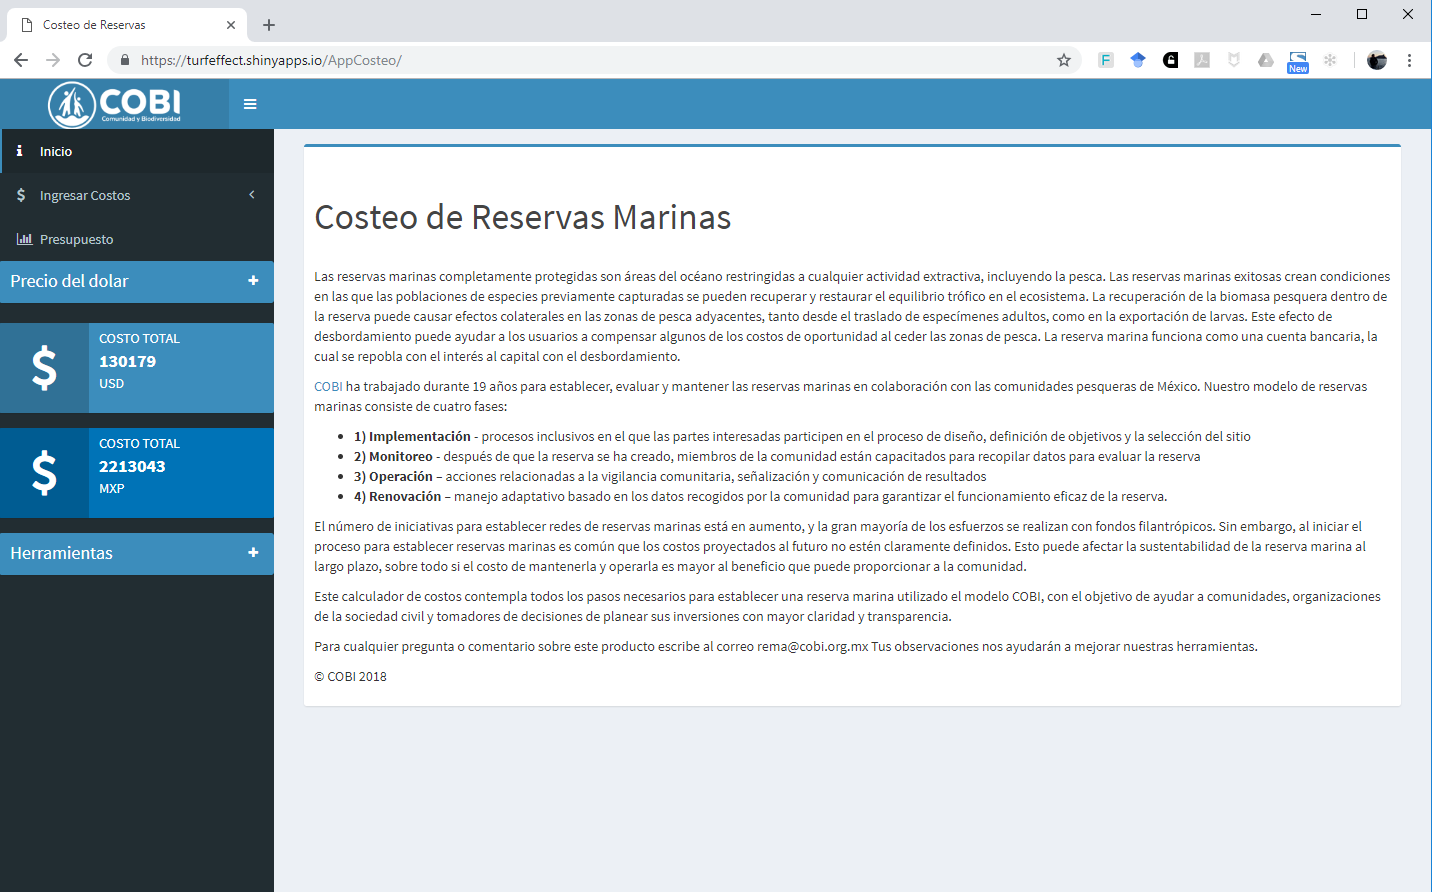
\includegraphics{C:/Users/JC/Documents/GitHub/curso_marea/img/app_costeo.PNG}
\caption{\label{fig:shiny-costeo}Shiny app de Costeo de Reservas, la app
está disponible en \url{https://turfeffect.shinyapps.io/AppCosteo/}}
\end{figure}

La app tiene dos secciones principales. Del lado izquierdo se muestra
una barra de herramientas que el usuario puede usar para navegar por las
secciones de \texttt{Ingresar\ costos} y \texttt{Presupuesto}, así como
ajustar el tipo de cambio, ver los cambios al total en tiempo real y
eventualmente descargar el presupuesto detallado u obtener un link para
compartir el estado de la app. La barra de herramientas se puede ocultar
y mostrar. La segunda sección es el área de trabajo, que al inicio
muestra una descripción similar a la del texto anterior.

Los costos unitarios y cantidades pueden ser editados en la sección de
\texttt{Ingresar\ costos}. La app de costeo contiene los rubros más
comunes de cada fase, además de presentar valores predeterminados y
editables para cada uno. Por ejemplo, navegando a
\texttt{Ingresar\ costos} \textgreater{}\textgreater{}
\texttt{Implementación} \textgreater{}\textgreater{}
\texttt{Definición\ de\ objetivos} \textgreater{}\textgreater{}
\texttt{Gasolina} veremos un valor de 1 en la columna de costos y 80 en
la columna de cantidades. En este caso, los costos están en dólares
estadounidenses, pero la app es agnóstica a una moneda en especial.

Este proceso se repite para cada una de las fases y rubros necesarios.
Una vez terminado, el usuario puede navegar a la sección de
\texttt{Presupuesto}. Aquí aparecen gráficas interactivas que muestran
en detalle los costos estimados por fase y concepto. Las gráficas pueden
editarse para mostrar los costos en otras unidades, cambiar el tamaño
del texto e incluso el esquema de colores.

Al confirmar que el presupuesto es correcto, el usuario puede ir a la
sección de herramientas y seleccionar la opción de
\texttt{Descargar\ presupuesto} que se muestra en el botón opaco. Esto
descargará un archivo de excel con el presupuesto detallado.

\hypertarget{uso-de-la-app}{%
\section{Uso de la App}\label{uso-de-la-app}}

\hypertarget{ejercicio}{%
\subsection{Ejercicio}\label{ejercicio}}

Supongamos que queremos diseñar e implementar (pero no monitorear ni
evaluar aún) una red de reservas marinas. ¿Cuál sería el costo total?

Responde las siguientes preguntas:

\begin{itemize}
\tightlist
\item
  ¿Cuál es el monto total en dólares?
\item
  ¿Cuál es el monto total en tu moneda local?
\end{itemize}

Al terminar, descarga una de las figuras después de incrementar el
tamaño de letra y cambiar el esquema de colores. Descarga también el
presupuesto detallado.

\hypertarget{pasos-sugeridos}{%
\subsection{Pasos sugeridos}\label{pasos-sugeridos}}

\begin{itemize}
\item
  Navega a la App de Costeo en
  \url{https://turfeffect.shinyapps.io/AppCosteo/}.
\item
  Inicia navegando a las secciones de \texttt{Monitoreo},
  \texttt{Operación} y \texttt{Renovación} y modificando todos los
  valores de las columnas de cantidades para que estén en 0. Ahora,
  regresa a la primera sección (\texttt{Implementación}) y modifica los
  valores de acuerdo a tus necesidades y conocimientos de costos.
\item
  Usa la caja de conversión de moneda y ajusta el valor de 1 dolar
  estadounidense al valor de tu moneda.
\item
  Ahora navega a la sección de \texttt{Presupuesto} y modifica las
  gráficas para que el tamaño de letra sea de 12 y el esquema de colores
  sea ``Pares''.
\item
  Al poner el cursos sobre las imágenes, aparecerá una barra de
  herramientas. Utiliza el ícono de una cámara para exportar la imagen
  como \texttt{*.PNG}.
\item
  En la sección de \texttt{Herramientas}, haz click en el boton de
  \texttt{Descargar\ presupuesto}.
\end{itemize}

\hypertarget{resultados}{%
\subsection{Resultados}\label{resultados}}

Mis resultados se muestran en la Figura \ref{fig:resultados-costeo}. En
mi caso, el proyecto de implementación tiene un costo de \$10,058 USD o
\$201,160 MXP. Puedo ver que la mayor parte de los costos (¡\$5,000
USD!) provienen de la estrategia de comunicación.

\begin{figure}
\centering
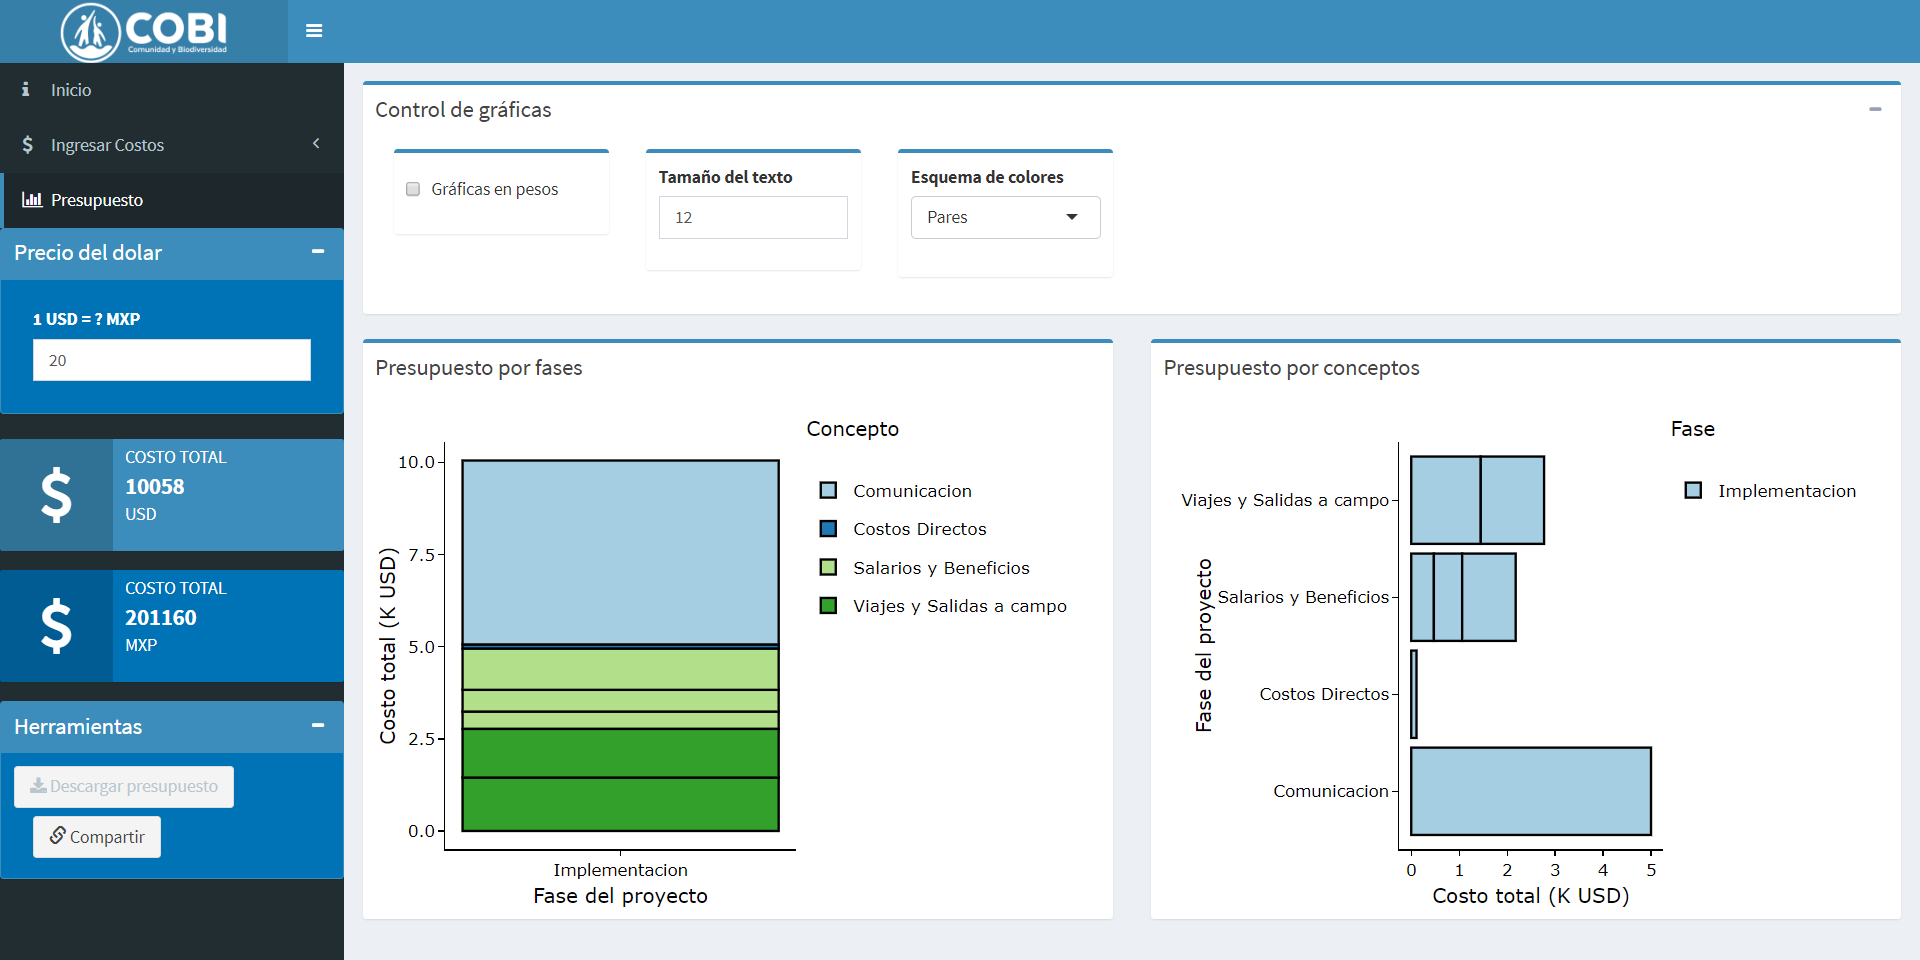
\includegraphics{C:/Users/JC/Documents/GitHub/curso_marea/img/app_costeo_estado.PNG}
\caption{\label{fig:resultados-costeo}Shiny app de Costeo de Reservas
mostrando los costos de diseño e implementación de una reserva.}
\end{figure}

\hypertarget{part-parte-ii}{%
\part{Parte II}\label{part-parte-ii}}

\hypertarget{antecedentes}{%
\chapter{Antecedentes}\label{antecedentes}}

La evaluación de reservas marinas no es algo nuevo. Sin embargo, muy
pocos trabajos las han evaluado utilizando técnicas que permitan
atribuir las diferencias observadas únicamente a las reservas. Por lo
tanto, es útil hacer una recapitulación de metodologías comúnmente
usadas antes de presentar la metodología utilizada por MAREA. Este
capítulo se enfoca en los indicadores y diseños muestreales, presentando
casos publicados en la literatura científica. Revisaremos tres diseños
de muestro generales que se han utilizado en la evaluación de reservas
marinas y discutiremos sus ventajas y desventajas, así como las
implicaciones en el manejo.

\hypertarget{antes-despues}{%
\section{Antes-Después}\label{antes-despues}}

Una de las formas más comunes de evaluar reservas marinas es mediante la
comparación de indicadores biológicos antes y después de la
implementación de la reserva. Por ejemplo \citet{wantiez_1997} evaluan
el efecto de las reservas marinas en las comunidades de peces de cinco
islas en Nueva Celadonia. El trabajo compara número de especies
(riqueza), número de organismos (densidades) y biomasa obtenidas para
nueve sitios en 1990 y 1994. Aunque las reservas fueron establecidas en
1989, la vigilancia y cumplimiento de las reglas comienza en 1990.
Aunque los autores identifican pocos cambios estadísticamente
significativos (solamente dos sitios muestran un incremento en
densidad), la metodología empleada ignora otras eventos que puedan haber
causado los efectos observados.

Por ejemplo, es posible que entre 1990 y 1994 hayan existido
intervenciones de manejo pesquero que redujeran el esfuerzo de pesca, el
ambiente pudo haber sufrido cambios que modificaran la productividad del
sistema, la sobrepesca de especies depredadoras o una serie de años de
buen reclutamiento podrían llevar a observar incrementos en densidad
\citep{szuwalski_2017, chavez_2003}. Para poder distinguir este tipo de
cambios, sería necesario un sitio control con el cual comparar
\citep{betti_2017}. Un sitio control podría ser un área con hábitat
similar al de la reserva, pero que presenta actividad pesquera.

La Figura \ref{fig:disenos}A muestra un caso hipotético de una
evaluación antes-después. En este caso, el indicador en la reserva
incrementó de 4 a 9 unidades. En esta evaluación, concluiríamos que la
reserva resulta en un incremento de 5 unidades al año. Sin embargo, la
línea azul muestra la tendencia temporal del control, mostrada en opaco
para representar que el evaluador no observa esa información.

\hypertarget{dentro-fuera}{%
\section{Dentro-Fuera}\label{dentro-fuera}}

Muchos trabajos evitan el problema de cambios temporales al evaluar
indicadores dentro y fuera de las zonas protegidas en una fecha única.
Por ejemplo, \citet{guidetti_2014} comparan 30 localidades del
Mediterráneo, que dividen en reservas estrictas, reservas intermedias y
áreas de pesca. El trabajo reporta diferencias en biomasa y riqueza
-pero no en densidades- con las reservas estrictas mostrando el mayor
efecto. Aunque el hábitat es similar entre grupos de sitios, esta
aproximación no toma encuenta las trayectorias o estados intrínsecos de
cada localidad ni otras inherentes diferencias espaciales que uno debe
tomar en cuenta.

En este caso, es posible que los sitios de pesca y reservas intermedias
siempre mostraran menor biomasa y riqueza, incluso antes de la
implementación de las reservas estrictas. También es posible que los
valores dentro de las reservas se hayan mantenido constantes desde su
creación, pero que las condiciones fuera de las reservas se hayan
deteriorado. Cualquiera de estas situaciones podría causar los patrones
observados, y un diseño muestreal que compare reservas contra zonas
control difícilmente podrá rechazar estas explicaciones alternas.

La Figura \ref{fig:disenos}B muestra un ejemplo de una evaluación donde
se compara dentro-fuera. Esta comparación indica que hay 4 unidades más
en la reserva que en el control. Este ejercicio ignora el hecho de que,
incluso antes de la implementación de la reserva, el sitio de reserva
presentaba una diferencia de 2 unidades. En este diseño muestreal el
evaluador no observa los valores históricos, por lo que aparecen en
opaco. Estos ejemplos muestran como los mismos datos pueden resultar en
estimaciones distintas, según la información que se tome en cuenta.
¿Entonces, cuál es el valor correcto? En realidad, ninguno de estos.

\hypertarget{antes-despues-dentro-fuera}{%
\section{Antes-Después-Dentro-Fuera}\label{antes-despues-dentro-fuera}}

Las secciones anteriores muestran que las evaluaciones antes-después o
dentro-fuera pueden ignorar factores importantes y, por lo tanto,
producir estimaciones incorrectas del efecto de una reserva. ¿Esto
quiere decir que las evaluaciones de \citet{wantiez_1997} y
\citet{guidetti_2014} están equivocadas? ¡Para nada! Sus conclusiones
indican que hay diferencias a través del tiempo, o entre sitios reserva
y sitios control, lo cual es cierto. Sin embargo, no es posible atribuir
la totalidad de las diferencias observadas a las reservas.

Cuando hablamos de intervenciones de manejo, nos interesa saber cual es
el \emph{impacto neto} de la intervención. En este sentido, y retomando
los ejemplos de las Figuras \ref{fig:disenos}A-B, queremos descomponer
el incremento de la reserva en sus tres partes: i) El incremento causado
por la evolución temporal, ii) el incremento \emph{aparente} causado por
las diferencias originales, y iii) el \emph{incremento neto} una vez que
tomamos en cuenta los anteriores.

Para poder medir el impacto neto, es necesario conocer las trayectorias
temporales (diferencia a través del tiempo) y las diferencias entre
sitios. Para esto, es necesario tener un diseño muestreal de
antes-después-control-impacto. En otras palabras, debemos tener
observaciones en la reserva y el control antes y después de la
implementación de la reserva. Una menor cantidad de trabajos han
evaluado reservas marinas con esta aproximación, pues requiere de muchos
datos \citep{moland_2013, villasenorderbez_2018}. Sin embargo, esto
permite atribuir parte de los cambios observados a las reservas.

Por ejemplo, en la Figura \ref{fig:disenos}C se muestran las mismas
tendencias que en los casos anteriores. En este caso, el evaluador
conoce las diferencias temporales de la reserva (de 4 a 9 = 5) y del
control (de 2 a 5 = 3). Com se mencionó antes, hay muchos factores que
podrían causar cambios a través del tiempo, incluso en la ausencia de
una reserva. En este caso, el sitio control presenta un incremento de 3
unidades. ¿Entonces, qué habría pasado con el sitio de reserva si no
hubiera recibido protección?

En teoría, el sitio debería de haber seguido la misma tendencia que el
sitio control. Es decir, debería de mostrar un incremento de 3 unidades.
La Figura \ref{fig:disenos}C muestra una línea roja punteada
representando este caso hipotético. Por lo tanto, la diferencia entre lo
observado (línea sólida) y lo que habría pasado (línea punteada) puede
ser atribuida a la protección. En otras palabras, de las 5 unidades de
diferencia que muestra la reserva, 3 son por otros factores y 2 por la
reserva. En este caso, podríamos entonces concluir que 2 de las unidades
son causadas por la reserva.

Esta técnica se conoce en econometría como \emph{Diferencia entre
Diferencias}, pues se calcula la diferencia a través del tiempo y a
través de sitios. El remanente de esta operación es entonces el efecto
neto observado. Desde luego, hay una serie de supuestos que debemos
tener en cuenta, como la factibilidad de que nuestro sitio control sea
realmente representativo. Además, al evaluar una reserva no tendremos
sólamente 4 puntos, pues por lo general usaremos datos de monitoreos
submarinos con muchas más observaciones. El siguiente capítulo (Capítulo
\ref{evaluacion-de-reservas}) habla más sobre los métodos de regresiones
utilizados en este caso, así como las otras dimensiones evaluadas por
MAREA.

\begin{figure}
\centering
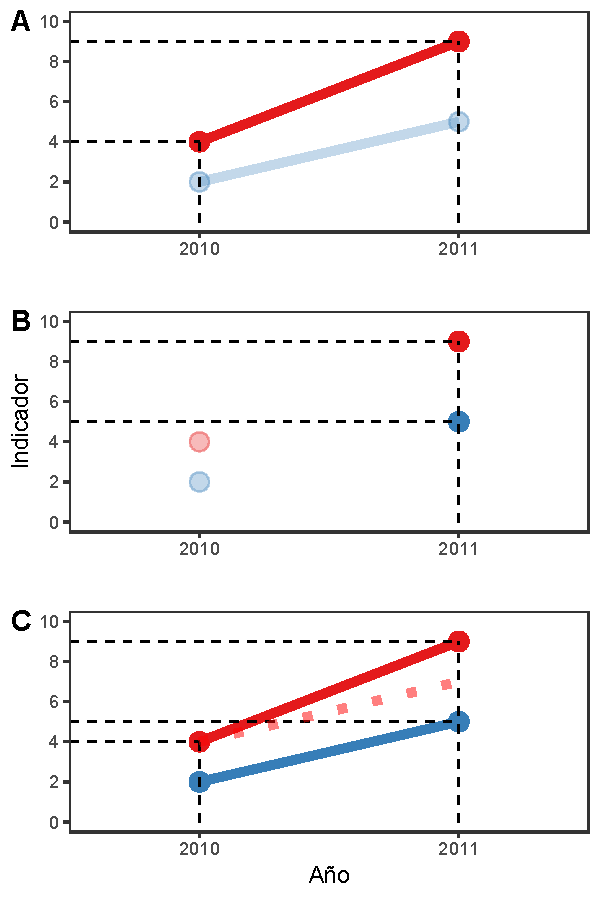
\includegraphics{evaluacion-reservas_files/figure-latex/disenos-1.pdf}
\caption{\label{fig:disenos}Ejemplos de evaluaciones antes-después (A),
dentro-fuera (B) y antes-después-dentro-fuera (C) para una reserva
hipotética implementada al final del 2010. Rojo representa reserva y
azul control, los colores opacos indican datos no observados u omitidos
en cada tipo de evaluación. La línea punteada en la figura C represente
la evolución que se hubiera esperado del sitio protegido si la reserva
no se hubiera implementado.}
\end{figure}

\hypertarget{evaluacion-de-reservas}{%
\chapter{Evaluación de reservas}\label{evaluacion-de-reservas}}

Las reservas marinas son sistemas socio-ecológicos complejos. Su
efectividad depende de las interacciones y combinaciones de factores
sociales y ambientales. Por muchos años, la ciencia de reservas marinas
sea ha enfocado en comprender los efectos ecológicos de estas áreas,
reportando aumentos en biomasa, riqueza y densidad de organismos o
beneficios de mitigación de cambio climático y protección ambiental
\citep{lester_2009, micheli_2012, giakoumi_2017, sala_2017, roberts_2017}.
Más recientemente, algunos trabajos se han enfocado en la relación entre
estructuras de governanza y aspectos socioeconómicos y la efectividad de
las reservas \citep{halpern_2013, lpezangarita_2014, mascia_2017}. Por
lo tanto, es importante que la evaluación de reservas tome en cuenta las
dimensiones ecológicas, socioeconómicas y de governanza.

La metodología propuesta e implementada en MAREA utiliza una serie de
indicadores de cada dimensión. Los indicadores sugeriods pueden ser
usados en función de los objetivos de la reserva o de otras preguntas de
interés. En este capítulo definimos los objetivos generales para los
cuales las reservas pueden ser implementadas y los indicadores sugeridos
para cada caso. Después explicamos a profundidad cómo MAREA utiliza el
análisis de Diferencias entre Diferencias presentado previamente en el
capítulo anterior (Capítulo \ref{antecedentes}).

\hypertarget{objetivos-e-indicadores}{%
\section{Objetivos e indicadores}\label{objetivos-e-indicadores}}

Como cualquier otra intervención de manejo, las reservas marinas deben
de tener objetivos claros\footnote{Idealmente, usaremos objetivos
  \href{https://en.wikipedia.org/wiki/SMART_criteria}{SMART}}. Los
objetivos nos ayudan a identificar los cambios que deseamos ver y, por
lo tanto, seleccionar indicadores para evaluar la efectividad de la
intervención.

En práctica, los objetivos suelen ser difusos y se encuentran escondidos
en documentos oficiales. Habrá ocasiones en las que diferentes agencias,
cuerpos o actores tengan percepciones distintas sobre los objetivos.
Otras, las reservas tendrán objetivos muy específicos (por ejemplo
``Duplicar la biomasa de mero en los primeros 10 años''). Por lo tanto,
es difícil generar una lista de todos los objetivos e indicadores
posibles.

En su lugar, la metodología desarrollada por
\citet{villasenorderbez_2018} e implementada en MAREA presenta una serie
de 7 objetivos generales a los cuales se asignan 25 indicadores
divididos en indicadores biológicos (n = 7), socioeconómicos (n = 3) y
de gobernanza (n = 15). Los 7 objetivos están inspirados en la
normatividad de las zonas de refugio pesquero \citep{nom}, pero agrupan
muchos otros objetivos más particulares.

\begin{table}

\caption{\label{tab:tabla-oi}Matriz de objetivos e indicadores. Cada columna representa un indicador biológico (B) o socioeconómico (S). Los indicadores de gobernanza no se muestran, pues sugerimos que todos sean utilizados sin importar el objetivo.}
\centering
\begin{tabular}[t]{lllllllllll}
\toprule
Objetivo & B1 & B2 & B3 & B4 & B5 & B6 & B7 & S1 & S2 & S3\\
\midrule
Evitar la sobreexplotación &  &  & x & x & x & x & x & x & x & x\\
Conservar especies bajo protección especial &  &  & x &  & x &  &  & x & x & x\\
Mantener procesos biológicos & x & x &  & x & x & x & x &  &  & x\\
Mejorar la productividad de las zonas de pesca &  &  &  & x & x &  & x & x & x & x\\
Preservar la biodiversidad y los ecosistemas & x & x &  & x & x & x & x &  &  & x\\
\addlinespace
Recuperar especies sobreexplotadas &  &  & x &  & x &  &  &  &  & x\\
Recuperar especies de inerés comercial &  &  & x &  & x &  &  &  &  & x\\
\bottomrule
\end{tabular}
\end{table}

La lista de indicadores presentada es el resultado de un proceso de
depuración de más de 40 indicadores iniciales obtenidos de la literatura
científica
\citep{halpern_2002, lester_2009, lester_2008, micheli_2012, halpern_2013, basurto_2013, leslie_2015}.
El proceso de selección incluyó pescadores, investigadores, gestores
ambientales y personal de agencias de gobeierno. Los indicadores fueron
elegidos según su facilidad de medición, la existencia de información
anterior y presencia de programas de monitoreo que los midan anualmente.
Además de separar explícitamente los indicadores en las ctegorías
previamente mencionadas, también hay una separación implícita entre
indicadores que cambian por efecto de la reserva (por ejemplo,
\textbf{B} - Biomasa) o indicadores que pueden explicar la efectividad
de la reserva, como \textbf{G5} - Pesca ilegal.

Los indicadores biológicos son:

\begin{itemize}
\tightlist
\item
  \textbf{B1} - Índice de diversidad de Shannon
\item
  \textbf{B2} - Riqueza de especies
\item
  \textbf{B3} - Densidad de organismos maduros (proporción de organismos
  mayores a la talla de primera maduréz)
\item
  \textbf{B4} - Densidad de organismos
\item
  \textbf{B5} - Presencia de una perturbación ambiental
\item
  \textbf{B6} - Nivel trófico medio
\item
  \textbf{B7} - Biomasa
\end{itemize}

Los indicadores socioeconómicos son:

\begin{itemize}
\tightlist
\item
  \textbf{S1} - Arribos totales
\item
  \textbf{S2} - Ingresos totales
\item
  \textbf{S3} - Oportunidades económicas alternativas a la pesca
\end{itemize}

Los indicadores de gobernanza son:

\begin{itemize}
\tightlist
\item
  \textbf{G1} - Acceso a la pesquería
\item
  \textbf{G2} - Número de pescadores
\item
  \textbf{G3} - Reconocimiento legal de la reserva
\item
  \textbf{G4} - Tipo de reserva
\item
  \textbf{G5} - Pesca ilegal
\item
  \textbf{G6} - Plan de manejo
\item
  \textbf{G7} - Procuración y vigilancia de la reserva
\item
  \textbf{G8} - Tamaño de la reserva
\item
  \textbf{G9} - Razonamiento para la localización de la reserva
\item
  \textbf{G10} - Presencia de organizaciones pesqueras
\item
  \textbf{G11} - Tipo de organizaciones pesqueras
\item
  \textbf{G12} - Representación
\item
  \textbf{G13} - Regulaciones internas
\item
  \textbf{G14} - Efectividad percibida
\item
  \textbf{G15} - Impacto social de la reserva
\end{itemize}

\hypertarget{analisis}{%
\section{Análisis}\label{analisis}}

Una vez definidos los indicadores, debemos establecer formas de
analizarlo. La metodología de colecta de datos no es parte central de
este manual, y ha sido descrita a detalle en otros trabajos
\citep{suman_2010, villaseorderbez_2017, villasenorderbez_2018}. En esta
sección describimos el análisis de Diferencias entre Diferencias
empleado para estimar el efecto de la reserva en los indicadores
biológicos y los análisis para indicadores socioeconómicos y de
gobernanza.

\hypertarget{inferencia-de-causalidad}{%
\subsection{Inferencia de causalidad}\label{inferencia-de-causalidad}}

Como se mencionó en la Sección \ref{antes-despues-dentro-fuera}, MAERA
usa un análisis de Diferencias en Diferencias. Pero ¿cómo funciona este
análisis cuando tenemos más de cuatro observciones? El análisis puede
hacerse por medio de una regresión lineal múltiple.

Retomando el ejemplo del capítulo anterior (Captítulo
\ref{antecedentes}), podemos imaginarnos un caso en el que tenemos dos
observaciones para cada sitio en cada periodo. En tal caso, podríamos
calcular el promedio de cada sitio en cada periodo. La Figura
\ref{fig:baci-multi} muestra las observaciones como puntos y los
promedios como líneas. En este caso, podríamos calcular la pendiente de
cada línea (esto es, el cambio en el tiempo) y así obtener el
contrafactual (línea punteada roja) y calcular el efecto de la reserva.

\begin{figure}
\centering
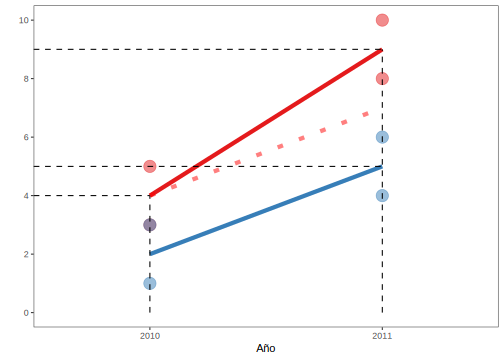
\includegraphics{evaluacion-reservas_files/figure-latex/baci-multi-1.pdf}
\caption{\label{fig:baci-multi}Diseño muestreal antes-despues-dentro-fuera
con dos observaciones por sitio y periodo (puntos). Las líneas sólidas
muestran las tendencias promedio de cada sitio con azul para el control
y rojo para la reserva. La línea punteada roja muestra el contrafactual
de la reserva. Las líneas punteadas negras horizontales y verticales
presentan los promedios de cada sitio y periodo.}
\end{figure}

Como el cambio a través del tiempo es básicamente una pendiente, podemos
usar una regersión lineal múltiple para obtener esos valores. En el caso
de Diferencias en Diferencias, nos interesan 3 cambios o pendientes: i)
La diferencia a través del tiempo y ii) La diferencia entre sitios y
iii) La diferencia entre estas diferencias.

Para calcular la diferencia a través del tiempo, podems definir una
variable llamada \(Post\) que tomará un valor \(Post = 0\) para todas
las observaciones antes de la implementación de la reserva y un valor de
\(Post = 1\) una vez que la reserva haya sido implementada. Al igual que
cuando comparamos 2011 contra 2010, la diferencia entre años o entre
\(Post\) será de 1 (\(2011 - 2010 = 1\); \(1 - 0 = 1\)).

Para obtener la diferencia entre sitios, definimos otra variablle
llamada \(Zona\) que tomará un valor de \(Zona = 0\) para las
observaciones realizadas en el control y un valor de \(Zona = 1\) para
las observaciones de la reserva. Finalmente, podemos ``interactuar''
(multiplicar) estas variables para generar un \emph{término de
interacción}, de tal manera que \(Zona \times Post = 0\) para todas las
observaciones del control y la observación de la reserva \textbf{antes}
de la implementación, y \(Zona \times Post = 1\) para las observaciones
de la reserva \textbf{después} de la implementación.

Por lo tanto, podemos definir un modelo lineal múltiple que contenga una
variable para el tiempo, una para la zona y otra para la interacción
entre estas, de la siguiente manera:

\begin{equation} 
I = \alpha + \beta_1Post + \beta_2Zona + \beta_3Zona \times Post + \epsilon
\label{eq:did}
\end{equation}

En esta especificación, estimamos los coeficientes \(\alpha\),
\(\beta_1\), \(\beta_2\) y \(\beta_3\) por medio de mínimos cuadrados
ordinarios. Estos coeficientes presentarán la siguiente información:

\begin{itemize}
\tightlist
\item
  \(\alpha\): promedio del indicador en la zona control antes de la
  implementación
\item
  \(\beta_1\): cambio a través del tiempo
\item
  \(\beta_2\): cambio a través de sitios
\item
  \(\beta_3\): restante del cambio entre reservas y sitios (este es el
  efecto de la reserva)
\end{itemize}

Esto es quivalente a un ANOVA de dos vías con un término de interacción.
La ventaja de hacerlo así es que no solamente podemos decir si hay o no
diferencias, si no que también inferir algo sobre la magnitud de estas
diferencias. La interpretación de estos coeficientes puede ser un poco
compleja, pero el siguiente ejemplo puede ayudarnos a aclarar dudas.
Ajustando el modelo lineal a los datos de la Figura
\ref{fig:baci-multi}, obtenemos los coeficientes mostrados en la Tabla
\ref{tab:reg}.

\begin{table}[!htbp] \centering 
  \caption{Coeficientes estimados mediante la regresión lineal múltiple.} 
  \label{tab:reg} 
\begin{tabular}{@{\extracolsep{5pt}}lc} 
\\[-1.8ex]\hline 
\hline \\[-1.8ex] 
 & \multicolumn{1}{c}{Variable dependiente} \\ 
\cline{2-2} 
\\[-1.8ex] & indicador \\ 
\hline \\[-1.8ex] 
 alpha & 2.000 (1.000) \\ 
  B1 & 3.000 (1.414) \\ 
  B2 & 2.000 (1.414) \\ 
  B3 & 2.000 (2.000) \\ 
 \hline \\[-1.8ex] 
Observations & 8 \\ 
R$^{2}$ & 0.867 \\ 
Residual Std. Error & 1.414 (df = 4) \\ 
F Statistic & 8.667$^{**}$ (df = 3; 4) \\ 
\hline 
\hline \\[-1.8ex] 
\textit{Note:}  & \multicolumn{1}{r}{$^{*}$p$<$0.1; $^{**}$p$<$0.05; $^{***}$p$<$0.01} \\ 
\end{tabular} 
\end{table}

La Tabla \ref{tab:reg} muestra los valores estimados para los
coeficientes. Los números entre paréntesis presentan el error estándar
al rededor de la estimación. Además, presenta la varianza explicada por
el modelo, en este caso con un valor de \(R^2 = 0.87\)\footnote{El
  modelo completo de MAREA incluye covariables que pueden ayudar a
  explicar mayor parte de la variación en los datos. Estos incluyen la
  profundidad, visibilidad y temperatura asociadas a cada observación.
  En este caso, 13\% de la variación faltante es debido a la
  manipulación manual de los datos, pero podríamos esperar que las
  covariables antes mencionadas expliquen algo de la variación en los
  datos.}.

Para interpretar los coeficientes, debemos sustituirlos en la ecuación
anterior. Por lo tanto, obtenemos lo siguiente:

\[
I = 2 + (3 \times Post) + (2\times Zona) + (2 \times Zona \times Post)
\]

Podemos usar esta acuación para calcular el valor promedio del indicador
\(I\) en cada sitio y cada perido según los valores de las variables
\(Post\), \(Zona\) y \(Zona \times Post\).

\hypertarget{valor-antes-en-el-control}{%
\subsubsection{Valor antes en el
control}\label{valor-antes-en-el-control}}

Primero, debemos definir los valores de las variables según el sitio y
periodo en el que estamos. Para los valores antes de la implementación
sabemos que \(Post = 0\). Para los valores del sitio control sabemos que
\(Zona = 0\). Sustituimos estos valores en la fórmula anterior y
obtenemos

\[
\begin{split}
I &= 2 + (3 \times 0) + (2\times 0) + (2 \times 0 \times 0) \\
I &= 2 + 0 + 0 + 0 \\
I &= 2
\end{split}
\]

Este ejercicio sugiere que el valor promedio del indicador en el control
antes de la intervención es de 2. La inspección visual de la Figura
\ref{fig:baci-multi} confirma esto.

\hypertarget{valor-despues-en-el-control}{%
\subsubsection{Valor después en el
control}\label{valor-despues-en-el-control}}

En este caso, \(Post = 1\) pero seguimos con \(Zona = 0\):

\[
\begin{split}
I &= 2 + (3 \times 1) + (2\times 0) + (2 \times 0 \times 0) \\
I &= 2 + 3 + 0 + 0 \\
I &= 5
\end{split}
\]

Ahora identificamos que el promedio del indicador en el control después
de la intervención es de 5, como lo vemos en la Figura
\ref{fig:baci-multi}.

\hypertarget{valor-antes-en-la-reserva}{%
\subsubsection{Valor antes en la
reserva}\label{valor-antes-en-la-reserva}}

Ahora, regresamos a tener \(Post = 0\) pero con \(Zona = 1\), pues
estamos en la reserva:

\[
\begin{split}
I &= 2 + (3 \times 0) + (2\times 1) + (2 \times 0 \times 0) \\
I &= 2 + 0 + 2 + 0 \\
I &= 4
\end{split}
\]

En este caso el promedio del indicador en la reserva antes de la
intervención es de 4 (Figura \ref{fig:baci-multi}).

\hypertarget{valor-despues-en-la-reserva}{%
\subsubsection{Valor después en la
reserva}\label{valor-despues-en-la-reserva}}

Para calcular el valor en el sitio de reserva después de la
intervención, tendremos \(Post = 1\) y \(Zona =1\). Hagamos el ejercicio
sin incluir el término de interacción por ahora:

\[
\begin{split}
I &= 2 + (3 \times 1) + (2\times 1) \\
I &= 2 + 3 + 2 \\
I &= 7
\end{split}
\]

¿Por qué obtenemos un valor de 7 si la reserva presenta un valor de 9
después de su implementación? En este caso, no hemos aún incluido el
valor del término de interacción, por lo que obtenemos el valor que la
reserva habría presentado si la reserva no se hubiera implementado. Este
es el contrafactual, mostrado como la línea punteada roja en la Figura
\ref{fig:baci-multi}. Al incluir el término de interacción, obtenemos:

\[
\begin{split}
I &= 2 + (3 \times 1) + (2\times 1) + (2\times 1 \times 1)\\
I &= 2 + 3 + 2 + 2\\
I &= 9
\end{split}
\]

El término de interacción captura la diferncia entre lo que debería de
haberse observado para la reserva y lo que realmente se observó. Es
decir, la diferencia entre las líneas rojas. Este término es el
\textbf{efecto de la reserva}. En este sentido, podemos entonces
concluir que una reserva marina causó un incremento de 2 unidades en el
indicador.

Aunque la regresión lineal y el álgebra pueden parecer complicados, en
la realidad todo puede implementarse con una línea de código (como
\texttt{lm(indicador\ \textasciitilde{}\ post\ *\ zona,\ data\ =\ datos)}).
Mejor aún, MAREA se encarga de generar las variables \(Post\) y
\(Zona\), ajustar el modelo, obtener los coeficientes y reportar los
resultados. En el siguiente capítulo (Capítulo \ref{uso-de-marea}),
describimos el uso de MAREA y demostramos que con 6 sencillos pasos
podemos evaluar todos los indicadores y obtener reportes para compartir.

\hypertarget{socioeconomicos-y-de-gobernanza}{%
\subsection{Socioeconómicos y de
gobernanza}\label{socioeconomicos-y-de-gobernanza}}

Ahora pasamos a describir el análisis de los indicadores socioeconómicos
y de gobernanza. Los primeros dos
\protect\hyperlink{objetivos-e-indicadores}{indicadores socioeconómicos}
son numéricos, pues representan los arribos (masa) e ingresos (dinero)
que generan las pesquerías de la comunidad. En este caso, no tenemos una
comunidad control, pero podemos aún inferir algo de los cambios mediante
una evaluación antes-después. Para esto, MAREA implementa una forma
reducida del modelo anterior:

\[
I = \alpha + \beta_1Post + \epsilon
\]

Lo anterior es equivalente a realizar una prueba t de student de dos
colas con muestras pareadas. Un valor de \(\beta_1 = 0\) indicaría que
no hay cambio en el indicador. Como se mencionó en el Capítulo
\ref{antecedentes}, una evaluación antes-después no toma en cuenta otros
factores exógenos y por lo tanto no podemos inferir causalidad. Sin
embargo, la información obtenida sigue siendo útil al evaluar las
reservas y el contexto social en el que se desarrollan.

La mayoría de los indicadores de gobernanza son cuantitativos. Por lo
tanto, no existe una evaluación numérica de estos. En su lugar,
\citet{villasenorderbez_2018} realizaron una revisión literaria para
identificar valores asociados a impactos positivos y negativos en la
reserva. Por ejemplo, el indicador \textbf{G5} - Pesca Ilegal nos indica
la presencia y / o el grado de pesca ilegal en la reserva, lo que
sabemos es detrimental.

\hypertarget{uso-de-marea}{%
\chapter{Uso de MAREA}\label{uso-de-marea}}

El Capítulo \ref{antecedentes} describió las diferentes formas de
evaluar reservas. El Capítulo \ref{evaluacion-de-reservas} describió la
lista de objetivos e indicadores y la metodología de MAREA. Este
capítulo presenta los pasos necesarios para evaluar una reserva con
MAREA. Comenzamos con una breve descripción de los datos, seguido de los
seis pasos necesarios para realizar la evaluación, la guía de
interpretación de resultados y una breve mención de las capacidades y
limitaciones de MAREA.

Los participantes del curso recibirán datos simulados para hacer los
ejercicios del Capítulo \ref{ejercicios-con-marea}. Sin embargo, el
usuario de MAREA puede descargar ejemplos de datos en la pestaña de
datos dentro de la aplicación.

\hypertarget{tipos-y-formatos-de-datos}{%
\section{Tipos y formatos de datos}\label{tipos-y-formatos-de-datos}}

Para poder usar MAREA sin problemas, es necesario que los datos tengan
el formato correcto y estén en formato comaseparado (\texttt{*.csv}).
Esta sección no pretende discutir en su totalidad el formato de datos.
En su lugar, mencionamos brevemente algunos detalles importantes sobre
el formato. La descripción detallada de los datos puede encontrarse en
el manual operativo de MAREA \citep{villaseorderbez_2017}.

\hypertarget{datos-biologicos}{%
\subsection{Datos biológicos}\label{datos-biologicos}}

MAREA utiliza tres tipos de datos: biológicos, socioeconómicos y de
gobernanza. Los datos biológicos provienen de los censos visuales hechos
en las zonas reserva y control. MAREA puede recibir dos bases biológicas
distintas, una de peces y otra de invertebrados. Las bases de datos
biológicos deberán contener, por lo menos, las columnas presentadas en
la Tabla \ref{tab:formato}.

\begin{table}

\caption{\label{tab:formato}Requerimientos mínimos para los nombres de columna de la base de datos biológicos.}
\centering
\begin{tabular}[t]{rlll}
\toprule
Orden de columna & Nombre de Columna & Descripción & Ejemplo\\
\midrule
1 & id & Un código único de identificación del transecto, compuesto por Dia, Mes, Ano, Comunidad, Sitio, Zona y Transecto, separado por guiones. & “01-01-2017-El Rosario-Punta Baja-Reserva-1” Hace referencia a el primer transecto en la reserva de Punta Baja, en El Rosario el primero de enero del 2017.\\
2 & Dia & El día de muestreo, un número entre 1 y 31 & “01” Para el primer día del mes y “31” para el último día del mes\\
3 & Mes & El mes de muestreo, dos dígitos  entre 1 y 12 & “01” Para enero y  “12” para diciembre\\
4 & Ano & El año de muestreo, expresado en 4 dígitos & 2017\\
5 & Comunidad & La comunidad asociada al sitio & El Rosario, en Baja California\\
\addlinespace
6 & Sitio & El nombre del sitio de muestreo & Punta Baja, que es un sitio de El Rosario\\
7 & Zona & Indica si es un sitio control o reserva & “Reserva” que indica que Punta Baja es una reserva\\
8 & RC & Los pares reserva-control & “Punta Baja - Lazaro” Indica que Lázaro es el control de Punta Baja\\
9 & Latitud & Latitud, expresada en grados decimales de por lo menos cuatro dígitos. No es necesario incluir N o S, esto se indica con los signos. & 28.4573 Para un sitio en el hemisferio norte; -18.5429 Para un sitio en el hemisferio sur\\
10 & Longitud & Longitud, expresada en grados decimales de por lo menos cuatro dígitos. No es necesario incluir E o W, esto se indica con los signos. & -115.3249 Para un sitio en el hemisferio oeste; 29.7812 Para un sitio en el hemisferio este\\
\addlinespace
11 & Transecto & Utilizar números enteros consecutivos para cada año y sitio. & 1\\
12 & Profundidad & Profundidad del transecto, en metros & 18\\
13 & Visibilidad & Visibilidad del transecto, en metros & 12\\
14 & Temperatura & Temperatura del fondo, en °C & 22\\
15 & GeneroEspecie & El nombre científico de la especie & Mycteroperca xenarcha\\
\addlinespace
16 & Longitud* & Longitud total, en centímetros & 20\\
17 & Abundancia & Número de organismos observados & 10\\
18 & a* & El índice ponderal en la ecuación de crecimiento alométrico & 0.00001\\
19 & b* & El factor alométrico en la ecuación de crecimiento alométrico & 3.02\\
20 & NivelTrofico* & El nivel trófico de la especie & 3.5\\
21 & LT50* & La longitud de primera madurez de la especie & 25\\
\bottomrule
\end{tabular}
\end{table}

Otras columnas importantes, pero no estrictamente necesaria podrían ser:

\begin{enumerate}
\def\labelenumi{\arabic{enumi}.}
\tightlist
\item
  BuzoMonitor: El nombre del buzo que colectó la información
\item
  Tiempo de inicio del transecto, en minutos de buceo
\item
  Tiempo final del transecto, en minutos de buceo
\item
  Habitat: Tipo de hábitat en el sitio
\item
  Genero: El género de la especie
\item
  Especie: La especie de la especie
\item
  NombreComun: Nombre común de la especie en español
\item
  Observaciones: Notas de interés u observaciones relevantes.
\end{enumerate}

De las columnas presentadas en la Tabla \ref{tab:formato}, la más
importante es \texttt{RC}. Esta columna es la que le indica a MAREA la
relación entre sitios reserva y control. En una base con más de 2
sitios, MAREA utiliza esta columna para saber qué sitios seleccionar al
hacer el análisis.

\hypertarget{datos-socioeconomicos}{%
\subsection{Datos socioeconómicos}\label{datos-socioeconomicos}}

Los datos socioeconómicos deberán contener información de los arribos e
ingresos anuales de cada especie. Además, deberán de contar con el
índice del precio al consumidor usado para normalizar los datos de
ingresos. Este índice puede ser obtenido por medio de la
\href{https://data.oecd.org/price/inflation-cpi.htm}{OCDE}.

\begin{table}

\caption{\label{tab:formato-soc}Requerimientos mínimos para los nombres de columna de la base de datos socioeconómicos.}
\centering
\begin{tabular}[t]{rlll}
\toprule
Orden de columna & Nombre de Columna & Descripción & Ejemplo\\
\midrule
1 & Ano & El año, expresado como un entero de 4 dígitos & 2017\\
2 & GeneroEspecie & El nombre científico del recurso & Panulirus interruptus\\
3 & NombreComun & El nombre común del recurso & Langosta roja\\
4 & ArribosTotales & Arribos anuales, en Kg & 40000\\
5 & IngresosTotales & Los ingresos generados, en pesos mexicanos & 10000000\\
\addlinespace
6 & CPI & Índice de Precio al Consumidor & 4.018617\\
7 & PrecioPromedio & Valor promedio en pesos / Kg & 250\\
\bottomrule
\end{tabular}
\end{table}

\hypertarget{gobernanza}{%
\subsection{Gobernanza}\label{gobernanza}}

Los datos de gobernanza se obtienen por medio de entrevistas y por lo
tanto son más complejos. Para facilitar el uso de la entrevista
sugerida, MAREA provee también una base de datos de Access que permite
capturas la información de las entrevistas y obtener la base con el
formato deseado. La base de Access se puede descargar en el menú lateral
de MAREA.

\hypertarget{notas-importantes}{%
\subsection{Notas importantes}\label{notas-importantes}}

\hypertarget{nombres-de-columnas}{%
\subsubsection{Nombres de columnas}\label{nombres-de-columnas}}

Los nombres de columnas deben de evitar utilizar caracteres especiales
(por ejemplo, ° / * \% \#) y otros que puedan hacer tu base imposible de
leer en otras plataformas, como los acentos y las diéresis. Los nombres
de columnas también deberán evitar espacios o paréntesis. Si una
variable está compuesta por dos palabras, deberás considerar renombrarla
a algo más simple. Por ejemplo ``número de transecto'' puede ser
simplemente ``transecto''. Alternativamente, si reducir el nombre de la
variable no es una opción, puedes escribirlo en formato ``camllo''
(i.e.~usar una mayúscula para cada primer letra de cada palabra). Por
ejemplo, la variable ``Genero especie'' se convierte en
``GeneroEspecie''. Además, omite utilizar unidades en los nombres de las
columnas. Como se explicó antes, los nombres de columnas deben de
incluir la menor información posible, y las unidades están disponibles
en los metadatos.

\hypertarget{comunidades-y-sitios}{%
\subsubsection{Comunidades y sitios}\label{comunidades-y-sitios}}

Algo importante para mantener presente es la necesidad de usar nombres
idénticos para comunidades y sitios de muestreo en toda la base de
datos. Por ejemplo, nombrar a la comunidad ``Santa Maria'' en la base de
datos biofísica, pero ``Sta. Maria'' en la base de datos socioeconómica
no es un procedimiento correcto. Como humanos, somos capaces de
identificar esas diferencias. Sin embargo, una computadora las
identificará como palabras estrictamente diferentes y causará que MAREA
falle.

\hypertarget{evaluacion-de-reservas-en-6-etapas}{%
\section{Evaluación de reservas en 6
etapas}\label{evaluacion-de-reservas-en-6-etapas}}

MAREA está diseñada para evaluar las reservas en seis pasos, divididos
por pestañas mostradas en la App. La Figura \ref{fig:shiny-marea}
presenta la pantalla de bienvenida de la aplicación.

\begin{figure}
\centering
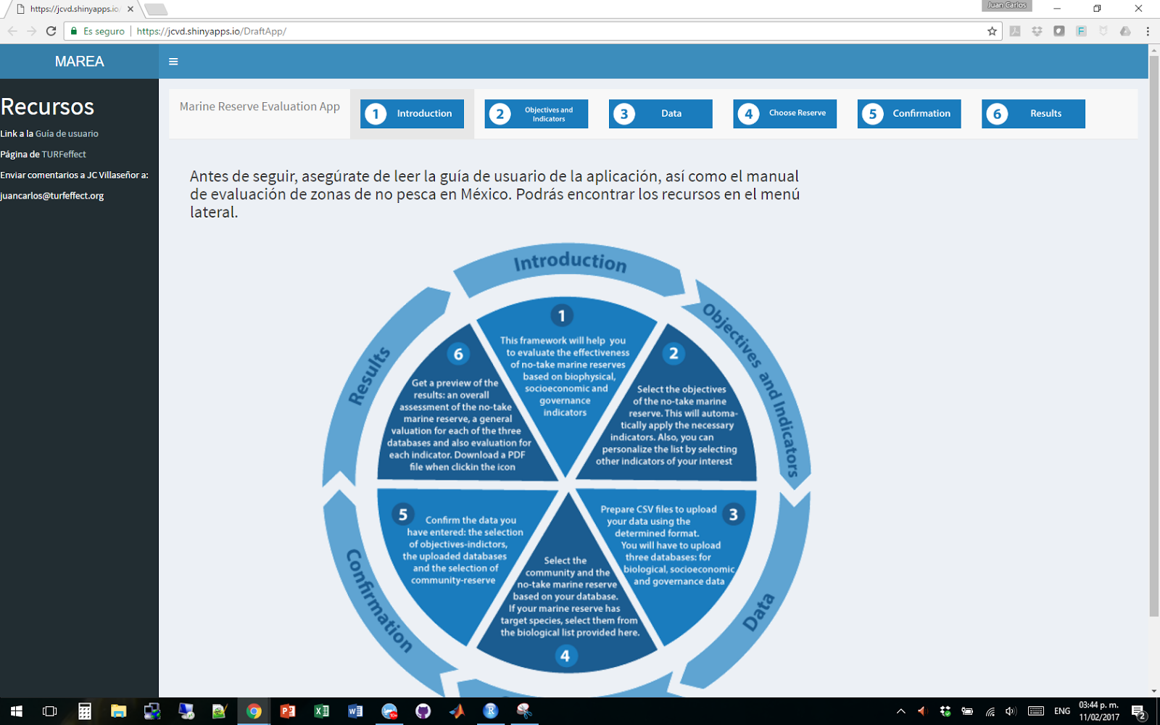
\includegraphics{C:/Users/JC/Documents/GitHub/curso_marea/img/Tab1.png}
\caption{\label{fig:shiny-marea}Aplicación para la evaluación de reservas
marinas, la app está disponible en
\url{https://turfeffect.shinyapps.io/marea/}}
\end{figure}

\begin{itemize}
\tightlist
\item
  La primer pestaña presenta una introducción a MAREA y un resumen del
  proceso de evaluación (Figura \ref{fig:workflow}).
\item
  El usuario navega a la segunda pestaña, donde especifica los objetivos
  de las reservas a evaluar y MAREA selecciona los objetivos según la
  Tabla \ref{tab:tabla-oi}. Recuerda que puedes modificar los
  indicadores seleccionados según tu interés.
\item
  La tercer pestaña permite al usuario cargar los datos y dercargar
  bases de ejemplo.
\item
  La cuarta pestaña utiliza la columna \texttt{RC} mencionada en la
  Tabla \ref{tab:formato} para presentar las reservas y controles que
  pueden ser evaluados, así como el año de implementación de la reserva,
  información sore el tamaño y la lista de especies objetivo a elegir.
\item
  La quinta pestaña presenta una confirmación de lo que el usuario
  seleccionó.
\item
  La sexta presenta los resultados de forma resumida con una tarjeta de
  puntuación y un botón para descargar el reporte en \texttt{*.pdf}.
\end{itemize}

\citet{villaseorderbez_2017} presenta una descripción detallada de cada
una de las pestañas.

\begin{figure}
\centering
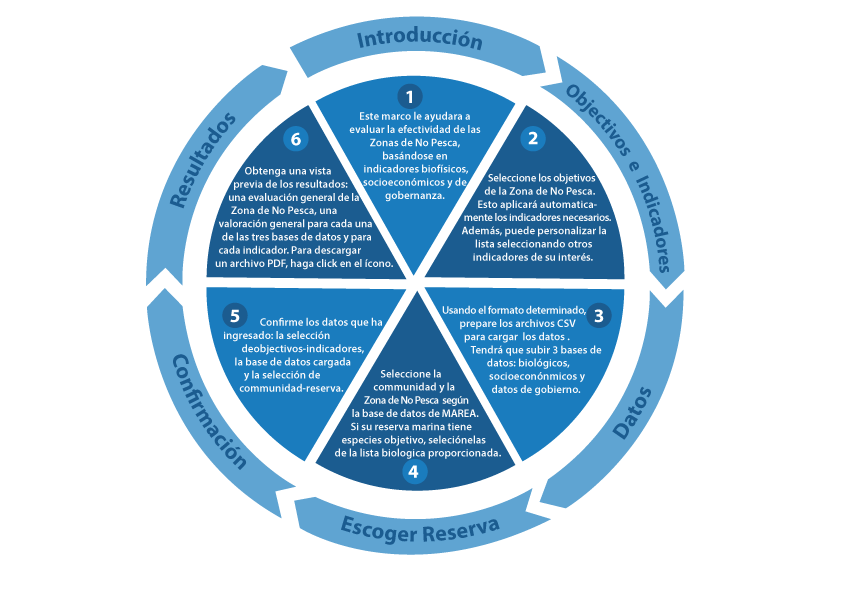
\includegraphics{C:/Users/JC/Documents/GitHub/curso_marea/img/workflow.png}
\caption{\label{fig:workflow}Diagrama de flujo de MAREA, explicando lo que
sucede en cada una de las 6 pestañas.}
\end{figure}

\hypertarget{interpretacion-de-resultados}{%
\section{Interpretación de
resultados}\label{interpretacion-de-resultados}}

El primer resultado es la tarjeta de puntiación (Figura
\ref{fig:resultados}), que presenta un recuadro coloreado para cada
indicador evaluado. El código de colores está indicado por la leyenda
mostrada en la Figura \ref{fig:leyenda}.

Para los indicadores biológicos, el color está dado por el signo y
significancia del efecto de la reserva (el \(\beta_3\) de la ecuación
\eqref{eq:did}). Para los socioeconómicos, el color está dado por el signo
y significancia de la pendiente de la regresión. Para los indicadores de
gobernanza, el rojo señala que el valor del indicador tiene efectos
negativos y el verde efectos positivos. Color amarillo para los
indicadores de gobernazna indica que la influencia del valor no está
clara o que el indicador no fue definido. El usuario puede descargar un
reporte en extenso al oprimir el botón \texttt{Descargar\ Reporte} en la
esquina superior derecha.

\begin{figure}
\centering
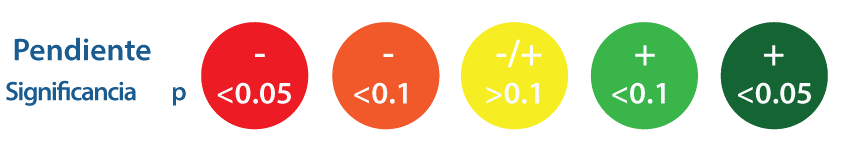
\includegraphics{C:/Users/JC/Documents/GitHub/curso_marea/img/leyenda.png}
\caption{\label{fig:leyenda}Leyenda usada para la interpretación de la
tarjeta de puntuación. Los colores indican la dirección del cambio y la
intensidad la significancia estadística.}
\end{figure}

\begin{figure}
\centering
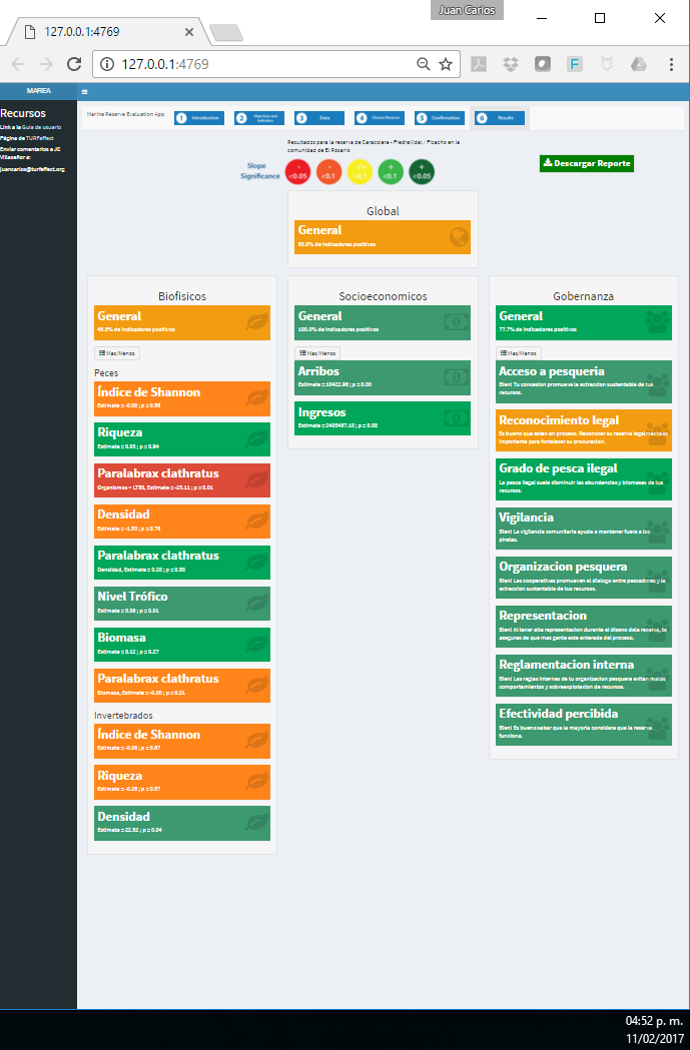
\includegraphics{C:/Users/JC/Documents/GitHub/curso_marea/img/AllResults.png}
\caption{\label{fig:resultados}Scorecard produced by MAREA for the ``La
Plana / Las Cuevas'' marine reserve in Isla Natividad, Mexico.}
\end{figure}

\hypertarget{part-parte-iii}{%
\part{Parte III}\label{part-parte-iii}}

\hypertarget{ejercicios-con-marea}{%
\chapter{Ejercicios con MAREA}\label{ejercicios-con-marea}}

Hola hola

\hypertarget{indicadores-biologicos}{%
\section{Indicadores biológicos}\label{indicadores-biologicos}}

\hypertarget{especie-objetivo}{%
\section{Especie objetivo}\label{especie-objetivo}}

\hypertarget{todos-los-indicadores}{%
\section{Todos los indicadores}\label{todos-los-indicadores}}

\hypertarget{datos-de-biometria}{%
\section{Datos de biometría}\label{datos-de-biometria}}

\hypertarget{mas-de-una-reserva-a-la-vez}{%
\section{Más de una reserva a la
vez}\label{mas-de-una-reserva-a-la-vez}}

\hypertarget{errores-y-soluciones}{%
\chapter{Errores y soluciones}\label{errores-y-soluciones}}

Hola

\hypertarget{especie-indicador-no-tiene-diseno-baci}{%
\section{Especie / Indicador no tiene diseño
BACI}\label{especie-indicador-no-tiene-diseno-baci}}

\hypertarget{diferentes-especies-en-bases-biologicas-vs-pesca}{%
\section{Diferentes especies en bases biológicas vs
pesca}\label{diferentes-especies-en-bases-biologicas-vs-pesca}}

\hypertarget{appendix-appendice}{%
\appendix \addcontentsline{toc}{chapter}{\appendixname}}


\hypertarget{datos-sinteticos}{%
\chapter{Datos sintéticos}\label{datos-sinteticos}}

Este apéndice muestra el código usado para obtener los datos sintéticos
del curso y el manual de evaluación. Primero, debemos definir una serie
de variables que contengan los valores predeterminados o rangos de
valores que cada variable puede tomar. Para los propósitos del curso,
generaremos únicamente información biológica y económica de peces.

\begin{Shaded}
\begin{Highlighting}[]
\CommentTok{# Cargamos los paquetes que necesitamos}
\KeywordTok{suppressPackageStartupMessages}\NormalTok{(\{}
  \KeywordTok{library}\NormalTok{(magrittr)}
  \KeywordTok{library}\NormalTok{(tidyverse)}
\NormalTok{\})}
\end{Highlighting}
\end{Shaded}

\begin{Shaded}
\begin{Highlighting}[]
\CommentTok{######################################}
\CommentTok{# Generar variables predeterminadas}
\CommentTok{######################################}

\CommentTok{# Las fechas estaran centradas en el dia 1 de cada mes}
\NormalTok{dia <-}\StringTok{ }\DecValTok{1}

\CommentTok{# Los muestreos ocurren aleatoriamente entre abril y junio}
\NormalTok{mes <-}\StringTok{ }\DecValTok{4}\OperatorTok{:}\DecValTok{6}

\CommentTok{# Generaremos datos del 200 al 2018}
\NormalTok{ano <-}\StringTok{ }\DecValTok{2000}\OperatorTok{:}\DecValTok{2018}

\CommentTok{# El estado va a ser NA}
\NormalTok{estado <-}\StringTok{ }\OtherTok{NA}

\CommentTok{# La comunidad imaginaria va a ser Las Positas}
\NormalTok{comunidad <-}\StringTok{ "Las Positas"}

\CommentTok{# En Las Positas hay 4 sitios, dos reservas y dos controles}
\CommentTok{# el tipo de sitio se define mas adelante}
\NormalTok{sitio <-}\StringTok{ }\KeywordTok{c}\NormalTok{(}\StringTok{"Las cruces"}\NormalTok{,}
           \StringTok{"Cerro prieto"}\NormalTok{,}
           \StringTok{"Calencho"}\NormalTok{,}
           \StringTok{"Popotla"}\NormalTok{)}

\CommentTok{# No es necesario definir el habitat}
\NormalTok{habitat <-}\StringTok{ }\OtherTok{NA}

\CommentTok{# La zona es determinada con esta funcion}
\NormalTok{zona <-}\StringTok{ }\ControlFlowTok{function}\NormalTok{(sitio)\{}
  \KeywordTok{ifelse}\NormalTok{(sitio }\OperatorTok\StringTok{ }\KeywordTok{c}\NormalTok{(}\StringTok{"Las cruces"}\NormalTok{,}
                      \StringTok{"Cerro prieto"}\NormalTok{),}
         \StringTok{"Reserva"}\NormalTok{,}
         \StringTok{"Control"}\NormalTok{)}
\NormalTok{\}}

\CommentTok{# Tipo de proteccion es NA}
\NormalTok{tipo_proteccion <-}\StringTok{ }\OtherTok{NA}

\CommentTok{# ANP es NA}
\NormalTok{ANP <-}\StringTok{ }\OtherTok{NA}

\CommentTok{# Lista de posibles buzos monitores}
\CommentTok{# (http://www.laff.bren.ucsb.edu/laff-network/alumni)}
\NormalTok{buzo_monitor <-}\StringTok{ }\KeywordTok{c}\NormalTok{(}\StringTok{"Caio Faro"}\NormalTok{,}
                  \StringTok{"Alexandra Smith"}\NormalTok{,}
                  \StringTok{"Diana Flores"}\NormalTok{, }
                  \StringTok{"Ignacia Rivera"}\NormalTok{,}
                  \StringTok{"Wagner Quiros"}\NormalTok{,}
                  \StringTok{"Gonzalo Banda"}\NormalTok{,}
                  \StringTok{"Camila Vargas"}\NormalTok{,}
                  \StringTok{"Diego Undurraga"}\NormalTok{,}
                  \StringTok{"Denise Garcia"}\NormalTok{,}
                  \StringTok{"Cristobal Libertad"}\NormalTok{,}
                  \StringTok{"Catalina Milagros"}\NormalTok{)}

\CommentTok{# Horas iniciales arbitrarias}
\NormalTok{hora_inicial <-}\StringTok{ }\KeywordTok{c}\NormalTok{(}\StringTok{"6:50"}\NormalTok{,}
                  \StringTok{"8:40"}\NormalTok{,}
                  \StringTok{"10:20"}\NormalTok{,}
                  \StringTok{"12:15"}\NormalTok{,}
                  \StringTok{"13:40"}\NormalTok{,}
                  \StringTok{"14:45"}\NormalTok{,}
                  \StringTok{"15:20"}\NormalTok{)}

\CommentTok{# Rango de profundidades iniciales posibles}
\NormalTok{profundidad_inicial <-}\StringTok{ }\DecValTok{5}\OperatorTok{:}\DecValTok{27}

\CommentTok{# Esta funcion inventa una profundidad final}
\CommentTok{# segun la profundidad inicial}
\NormalTok{profundidad_final <-}\StringTok{ }\ControlFlowTok{function}\NormalTok{(profundidad_inicial)\{}
  \KeywordTok{round}\NormalTok{(profundidad_inicial }\OperatorTok{+}\StringTok{ }\KeywordTok{rnorm}\NormalTok{(}\DataTypeTok{n =} \DecValTok{1}\NormalTok{, }\DataTypeTok{mean =} \DecValTok{0}\NormalTok{, }\DataTypeTok{sd =} \DecValTok{1}\NormalTok{),}
        \DataTypeTok{digits =} \DecValTok{1}\NormalTok{)}
\NormalTok{\}}

\CommentTok{# Rango de temperaturas}
\NormalTok{temperatura <-}\StringTok{ }\DecValTok{25}\OperatorTok{:}\DecValTok{27}

\CommentTok{# Rango de visibilidades}
\NormalTok{visibilidad <-}\StringTok{ }\DecValTok{3}\OperatorTok{:}\DecValTok{12}

\CommentTok{# Corriente es NA}
\NormalTok{corriente <-}\StringTok{ }\OtherTok{NA}

\CommentTok{# Numeros de transectos}
\NormalTok{transecto <-}\StringTok{ }\DecValTok{1}\OperatorTok{:}\DecValTok{12}

\CommentTok{# Crear un origen en comun para las secuencias aleatorias}
\KeywordTok{set.seed}\NormalTok{(}\DecValTok{42}\NormalTok{)}

\CommentTok{# De la lista de especies filtramos para tener}
\CommentTok{# especies menores a 160 cm y que tengan todos}
\CommentTok{# los parametros de a,b, NT y Lmax}
\NormalTok{spp <-}\StringTok{ }\NormalTok{MPAtools}\OperatorTok{::}\NormalTok{species_bio }\OperatorTok
\StringTok{  }\KeywordTok{filter}\NormalTok{(Lmax }\OperatorTok{<}\StringTok{ }\DecValTok{160}\NormalTok{) }\OperatorTok\StringTok{ }
\StringTok{  }\KeywordTok{select}\NormalTok{(GeneroEspecie, a, b, NT, Lmax) }\OperatorTok
\StringTok{  }\KeywordTok{drop_na}\NormalTok{() }\OperatorTok\StringTok{ }
\StringTok{  }\KeywordTok{sample_n}\NormalTok{(}\DecValTok{15}\NormalTok{)}

\CommentTok{# Crear un vector con todas las especies}
\NormalTok{genero_especie <-}\StringTok{ }\NormalTok{spp}\OperatorTok{$}\NormalTok{GeneroEspecie}

\CommentTok{# Esta funcion inventa una talla observada con una }
\CommentTok{# distribucion normal con promedio = la mitad entre}
\CommentTok{# 0 y la longitud maxima reportada y desviacion}
\CommentTok{# estandar = 0.3 * el promedio}
\NormalTok{tallas <-}\StringTok{ }\ControlFlowTok{function}\NormalTok{(spp, generoespecie)\{}
  
  \CommentTok{# calcular talla media}
\NormalTok{  talla <-}\StringTok{ }\NormalTok{spp }\OperatorTok\StringTok{ }
\StringTok{    }\KeywordTok{filter}\NormalTok{(GeneroEspecie }\OperatorTok{==}\StringTok{ }\NormalTok{generoespecie) }\OperatorTok\StringTok{ }
\StringTok{    }\NormalTok{Lmax }\OperatorTok{/}\StringTok{ }\DecValTok{2}
  
  \CommentTok{# obtener ruido al rededor de la talla media}
\NormalTok{  noise <-}\StringTok{ }\KeywordTok{rnorm}\NormalTok{(}\DataTypeTok{n =} \DecValTok{1}\NormalTok{, }\DataTypeTok{mean =} \DecValTok{0}\NormalTok{, }\DataTypeTok{sd =} \FloatTok{0.3} \OperatorTok{*}\StringTok{ }\NormalTok{talla }\OperatorTok{/}\StringTok{ }\DecValTok{2}\NormalTok{)}
  
  \CommentTok{# Redondear para evitar decimales}
  \KeywordTok{round}\NormalTok{(talla }\OperatorTok{+}\StringTok{ }\NormalTok{noise)}
\NormalTok{\}}

\CommentTok{# Esta funcion regresa la abundancia de la especie}
\CommentTok{# que es un numero que sigue una distribucion de}
\CommentTok{# poisson con Lambda = 12}
\NormalTok{mean_sp <-}\StringTok{ }\ControlFlowTok{function}\NormalTok{(generoespecie)\{}
  \KeywordTok{rpois}\NormalTok{(}\DataTypeTok{n =} \DecValTok{1}\NormalTok{, }\DataTypeTok{lambda =} \DecValTok{12}\NormalTok{)}
\NormalTok{\}}

\CommentTok{# Esta funcion regresa el par RC para cada sitio}
\NormalTok{rc <-}\StringTok{ }\ControlFlowTok{function}\NormalTok{(sitio)\{}
  \KeywordTok{ifelse}\NormalTok{(sitio }\OperatorTok\StringTok{ }\KeywordTok{c}\NormalTok{(}\StringTok{"Las cruces"}\NormalTok{,}
                      \StringTok{"Calencho"}\NormalTok{),}
         \StringTok{"Las cruces - Calencho"}\NormalTok{,}
         \StringTok{"Cerro prieto - Popotla"}\NormalTok{)}
\NormalTok{\}}
\end{Highlighting}
\end{Shaded}

\begin{Shaded}
\begin{Highlighting}[]
\CommentTok{######################################}
\CommentTok{# Simular datos}
\CommentTok{######################################}

\CommentTok{# Crear un data.frame vacio}
\NormalTok{datos <-}\StringTok{ }\KeywordTok{tibble}\NormalTok{(}\DataTypeTok{Dia =} \OtherTok{NA}\NormalTok{,}
                \DataTypeTok{Mes =} \OtherTok{NA}\NormalTok{,}
                \DataTypeTok{Ano =} \OtherTok{NA}\NormalTok{,}
                \DataTypeTok{Estado =} \OtherTok{NA}\NormalTok{,}
                \DataTypeTok{Comunidad =} \OtherTok{NA}\NormalTok{,}
                \DataTypeTok{Sitio =} \OtherTok{NA}\NormalTok{,}
                \DataTypeTok{Latitud =} \OtherTok{NA}\NormalTok{,}
                \DataTypeTok{Longitud =} \OtherTok{NA}\NormalTok{,}
                \DataTypeTok{Habitat =} \OtherTok{NA}\NormalTok{,}
                \DataTypeTok{Zona =} \OtherTok{NA}\NormalTok{,}
                \DataTypeTok{TipoProteccion =} \OtherTok{NA}\NormalTok{,}
                \DataTypeTok{ANP =} \OtherTok{NA}\NormalTok{,}
                \DataTypeTok{BuzoMonitor =} \OtherTok{NA}\NormalTok{,}
                \DataTypeTok{HoraInicial =} \OtherTok{NA}\NormalTok{,}
                \DataTypeTok{ProfundidadInicial =} \OtherTok{NA}\NormalTok{,}
                \DataTypeTok{ProfundidadFinal =} \OtherTok{NA}\NormalTok{,}
                \DataTypeTok{Temperatura =} \OtherTok{NA}\NormalTok{,}
                \DataTypeTok{Visibilidad =} \OtherTok{NA}\NormalTok{,}
                \DataTypeTok{Corriente =} \OtherTok{NA}\NormalTok{,}
                \DataTypeTok{Transecto =} \OtherTok{NA}\NormalTok{,}
                \DataTypeTok{Genero =} \OtherTok{NA}\NormalTok{,}
                \DataTypeTok{Especie =} \OtherTok{NA}\NormalTok{,}
                \DataTypeTok{GeneroEspecie =} \OtherTok{NA}\NormalTok{,}
                \DataTypeTok{Sexo =} \OtherTok{NA}\NormalTok{,}
                \DataTypeTok{Talla =} \OtherTok{NA}\NormalTok{,}
                \DataTypeTok{ClaseTalla =} \OtherTok{NA}\NormalTok{,}
                \DataTypeTok{Abundancia =} \OtherTok{NA}\NormalTok{,}
                \DataTypeTok{RC =} \OtherTok{NA}\NormalTok{)}

\CommentTok{# Definir un ciclo para iterar cada año}
\ControlFlowTok{for}\NormalTok{(i }\ControlFlowTok{in}\NormalTok{ ano)\{}
  \CommentTok{# El ano es determinado por el ciclo}
\NormalTok{  Ano <-}\StringTok{ }\NormalTok{i}
  
  \CommentTok{# El estado es constante}
\NormalTok{  Estado <-}\StringTok{ }\NormalTok{estado}
  
  \CommentTok{# La comunidad es constante}
\NormalTok{  Comunidad <-}\StringTok{ }\NormalTok{comunidad}
  
  \CommentTok{# Definir un ciclo para iterar cada sitio}
  \ControlFlowTok{for}\NormalTok{(j }\ControlFlowTok{in}\NormalTok{ sitio)\{}
    
    \CommentTok{# El sitio es determinado por el ciclo}
\NormalTok{    Sitio <-}\StringTok{ }\NormalTok{j}
    
    \CommentTok{#La latitud y longitud son NAs}
\NormalTok{    Latitud <-}\StringTok{ }\OtherTok{NA}
\NormalTok{    Longitud <-}\StringTok{ }\OtherTok{NA}
    
    \CommentTok{# El habitat es constante (NA)}
\NormalTok{    Habitat <-}\StringTok{ }\NormalTok{habitat}
    
    \CommentTok{# Definir la zona segun la funcion anterior}
\NormalTok{    Zona <-}\StringTok{ }\KeywordTok{zona}\NormalTok{(j)}
    
    \CommentTok{# El tipo de proteccion es constante (NA)}
\NormalTok{    TipoProteccion <-}\StringTok{ }\NormalTok{tipo_proteccion}
    
    \CommentTok{# El ANP es constante (NA)}
\NormalTok{    ANP <-}\StringTok{ }\NormalTok{ANP}
    
    \CommentTok{# Definir un ciclo para iterar cada transecto}
    \ControlFlowTok{for}\NormalTok{(k }\ControlFlowTok{in}\NormalTok{ transecto)\{}
      
\NormalTok{      Dia <-}\StringTok{ }\NormalTok{dia}
      
      \CommentTok{# Aleatoriamente muestreamos un mes de la lista anterior}
\NormalTok{      Mes <-}\StringTok{ }\KeywordTok{sample}\NormalTok{(}\DataTypeTok{x =}\NormalTok{ mes,}
                    \DataTypeTok{size =}\NormalTok{ 1L)}
      
      \CommentTok{# Escoger aleatoriamente un buzo monitor}
\NormalTok{      BuzoMonitor <-}\StringTok{ }\KeywordTok{sample}\NormalTok{(}\DataTypeTok{x =}\NormalTok{ buzo_monitor,}
                            \DataTypeTok{size =}\NormalTok{ 1L)}
      
      \CommentTok{# Escoger aleatoriamente la hora inicial}
\NormalTok{      HoraInicial <-}\StringTok{ }\NormalTok{hora_inicial[}\KeywordTok{sample}\NormalTok{(}\DataTypeTok{x =} \DecValTok{1}\OperatorTok{:}\DecValTok{7}\NormalTok{,}
                                         \DataTypeTok{size =}\NormalTok{ 1L)]}
      
      \CommentTok{# Escoger alteatoriamente la profundidad inicial}
\NormalTok{      ProfundidadInicial <-}\StringTok{ }\KeywordTok{sample}\NormalTok{(}\DataTypeTok{x =}\NormalTok{ profundidad_inicial,}
                                   \DataTypeTok{size =}\NormalTok{ 1L)}
      
      \CommentTok{# Calcular la profundidad final segun la funcion anterior}
\NormalTok{      ProfundidadFinal <-}\StringTok{ }\KeywordTok{profundidad_final}\NormalTok{(ProfundidadInicial)}
      
      \CommentTok{# Escoger una temperatura alteatoria}
\NormalTok{      Temperatura <-}\StringTok{ }\KeywordTok{sample}\NormalTok{(}\DataTypeTok{x =}\NormalTok{ temperatura,}
                            \DataTypeTok{size =}\NormalTok{ 1L)}
      
      \CommentTok{# Escoger una visibilidad aleatoria}
\NormalTok{      Visibilidad <-}\StringTok{ }\KeywordTok{sample}\NormalTok{(}\DataTypeTok{x =}\NormalTok{ visibilidad,}
                            \DataTypeTok{size =}\NormalTok{ 1L)}
      
      \CommentTok{# Corriente es NA}
\NormalTok{      Corriente <-}\StringTok{ }\OtherTok{NA}
      
      \CommentTok{# El transecto esta determinado por el ciclo}
\NormalTok{      Transecto <-}\StringTok{ }\NormalTok{k}
      
      \CommentTok{# Obtener un numero aleatorio para la riqueza}
\NormalTok{      n_spp <-}\StringTok{ }\KeywordTok{runif}\NormalTok{(}\DataTypeTok{n =} \DecValTok{1}\NormalTok{, }\DataTypeTok{min =} \DecValTok{0}\NormalTok{, }\DataTypeTok{max =} \DecValTok{10}\NormalTok{) }\OperatorTok\StringTok{ }
\StringTok{        }\KeywordTok{as.integer}\NormalTok{()}
      
      \CommentTok{# Muestrear la lista de especies para obtener las}
      \CommentTok{# observadas en este transecto}
\NormalTok{      GeneroEspecie <-}\StringTok{ }\KeywordTok{sample}\NormalTok{(genero_especie,}
                              \DataTypeTok{size =}\NormalTok{ n_spp)}
      \CommentTok{# Sexo es NA}
\NormalTok{      Sexo <-}\StringTok{ }\OtherTok{NA}
      
      \CommentTok{# La funcion rc me dice los pares RC}
\NormalTok{      RC <-}\StringTok{ }\KeywordTok{rc}\NormalTok{(Sitio)}
      
      \CommentTok{# Definir un ciclo para iterar cada especie}
      \ControlFlowTok{for}\NormalTok{(l }\ControlFlowTok{in}\NormalTok{ GeneroEspecie)\{}
        
        \CommentTok{# Separar genero y especie}
\NormalTok{        Genero <-}\StringTok{ }\KeywordTok{str_split}\NormalTok{(l, }\StringTok{" "}\NormalTok{)[[}\DecValTok{1}\NormalTok{]][[}\DecValTok{1}\NormalTok{]]}
\NormalTok{        Especie <-}\StringTok{ }\KeywordTok{str_split}\NormalTok{(l, }\StringTok{" "}\NormalTok{)[[}\DecValTok{1}\NormalTok{]][[}\DecValTok{2}\NormalTok{]]}
        
        \CommentTok{# Obtener un numero aleatorio entre 1 y 5 para}
        \CommentTok{# definir el numero de grupos de tallas observados}
\NormalTok{        nobs <-}\StringTok{ }\KeywordTok{sample}\NormalTok{(}\DataTypeTok{x =} \DecValTok{1}\OperatorTok{:}\DecValTok{5}\NormalTok{, }\DataTypeTok{size =}\NormalTok{ 1L)}
        
        \CommentTok{# Definir un ciclo para iterar cada grupo de}
        \CommentTok{# observaciones de una spp}
        \ControlFlowTok{for}\NormalTok{(m }\ControlFlowTok{in} \DecValTok{1}\OperatorTok{:}\NormalTok{nobs)\{}
          
          \CommentTok{# Escoger una talla aleatoria segun la funcion anterior}
\NormalTok{          Talla <-}\StringTok{ }\KeywordTok{tallas}\NormalTok{(}\DataTypeTok{spp =}\NormalTok{ spp, }\DataTypeTok{generoespecie =}\NormalTok{ l)}
          
          \CommentTok{# Clase talla es constante (NA)}
\NormalTok{          ClaseTalla <-}\StringTok{ }\OtherTok{NA}
          
          \CommentTok{# Muestrear una abundanciasegun la funcion}
\NormalTok{          Abundancia <-}\StringTok{ }\KeywordTok{mean_sp}\NormalTok{(}\DataTypeTok{generoespecie =}\NormalTok{ l)}
          
          \CommentTok{# Juntar las observaciones de este grupo de tallas}
\NormalTok{          datos_ijklm <-}\StringTok{ }\KeywordTok{tibble}\NormalTok{(Dia,}
\NormalTok{                                Mes,}
\NormalTok{                                Ano,}
\NormalTok{                                Estado,}
\NormalTok{                                Comunidad,}
\NormalTok{                                Sitio,}
\NormalTok{                                Latitud,}
\NormalTok{                                Longitud,}
\NormalTok{                                Habitat,}
\NormalTok{                                Zona,}
\NormalTok{                                TipoProteccion,}
\NormalTok{                                ANP,}
\NormalTok{                                BuzoMonitor, }
\NormalTok{                                HoraInicial,}
\NormalTok{                                ProfundidadInicial,}
\NormalTok{                                ProfundidadFinal,}
\NormalTok{                                Temperatura,}
\NormalTok{                                Visibilidad,}
\NormalTok{                                Corriente,}
\NormalTok{                                Transecto,}
\NormalTok{                                Genero,}
\NormalTok{                                Especie,}
                                \DataTypeTok{GeneroEspecie =}\NormalTok{ l,}
\NormalTok{                                Sexo,}
\NormalTok{                                Talla,}
\NormalTok{                                ClaseTalla,}
\NormalTok{                                Abundancia,}
\NormalTok{                                RC)}
          
\NormalTok{          datos <-}\StringTok{ }\KeywordTok{rbind}\NormalTok{(datos, datos_ijklm)}
\NormalTok{        \} }\CommentTok{# Fin nobs}
\NormalTok{      \} }\CommentTok{# Fin especie}
\NormalTok{    \} }\CommentTok{# Fin transecto}
\NormalTok{  \} }\CommentTok{# Fin sitio}
\NormalTok{\} }\CommentTok{# Fin años}

\CommentTok{# Borrar los NAs originales y agrupar grupos de}
\CommentTok{# talla en caso de que esten duplicados}
\NormalTok{datos }\OperatorTok
\StringTok{  }\KeywordTok{drop_na}\NormalTok{(dia) }\OperatorTok\StringTok{ }
\StringTok{  }\KeywordTok{group_by}\NormalTok{(Dia, Mes, Ano, Estado, Comunidad, Sitio, Latitud,}
\NormalTok{           Longitud, Habitat, Zona, TipoProteccion, ANP,}
\NormalTok{           BuzoMonitor,  HoraInicial, ProfundidadInicial,}
\NormalTok{           ProfundidadFinal, Temperatura, Visibilidad, Corriente,}
\NormalTok{           Transecto, Genero, Especie, GeneroEspecie, Sexo,}
\NormalTok{           Talla, ClaseTalla, RC) }\OperatorTok\StringTok{ }
\StringTok{  }\KeywordTok{summarize}\NormalTok{(}\DataTypeTok{Abundancia =} \KeywordTok{sum}\NormalTok{(Abundancia, }\DataTypeTok{na.rm =}\NormalTok{ T)) }\OperatorTok\StringTok{ }
\StringTok{  }\KeywordTok{ungroup}\NormalTok{() }\OperatorTok\StringTok{ }
\StringTok{  }\KeywordTok{select}\NormalTok{(Dia, Mes, Ano, Estado, Comunidad, Sitio, Latitud,}
\NormalTok{           Longitud, Habitat, Zona, TipoProteccion, ANP,}
\NormalTok{           BuzoMonitor,  HoraInicial, ProfundidadInicial,}
\NormalTok{           ProfundidadFinal, Temperatura, Visibilidad, Corriente,}
\NormalTok{           Transecto, Genero, Especie, GeneroEspecie, Sexo,}
\NormalTok{           Talla, ClaseTalla, Abundancia, RC)}
\end{Highlighting}
\end{Shaded}

\begin{Shaded}
\begin{Highlighting}[]
\CommentTok{# Graficar los datos}
\KeywordTok{ggplot}\NormalTok{(}\DataTypeTok{data =}\NormalTok{ datos,}
       \DataTypeTok{mapping =} \KeywordTok{aes}\NormalTok{(}\DataTypeTok{x =}\NormalTok{ Ano, }\DataTypeTok{y =}\NormalTok{ Abundancia,}
                     \DataTypeTok{color =}\NormalTok{ Zona, }\DataTypeTok{group =}\NormalTok{ Sitio, }\DataTypeTok{linetype =}\NormalTok{ RC)) }\OperatorTok{+}
\StringTok{  }\KeywordTok{geom_point}\NormalTok{(}\DataTypeTok{alpha =} \FloatTok{0.5}\NormalTok{, }\DataTypeTok{size =} \FloatTok{0.5}\NormalTok{) }\OperatorTok{+}
\StringTok{  }\KeywordTok{stat_summary}\NormalTok{(}\DataTypeTok{geom =} \StringTok{"line"}\NormalTok{, }\DataTypeTok{fun.y =} \StringTok{"mean"}\NormalTok{, }\DataTypeTok{size =} \DecValTok{1}\NormalTok{) }\OperatorTok{+}
\StringTok{  }\KeywordTok{facet_wrap}\NormalTok{(}\OperatorTok{~}\NormalTok{GeneroEspecie, }\DataTypeTok{ncol =} \DecValTok{3}\NormalTok{, }\DataTypeTok{scales =} \StringTok{"free_y"}\NormalTok{) }\OperatorTok{+}
\StringTok{  }\NormalTok{startR}\OperatorTok{::}\KeywordTok{ggtheme_plot}\NormalTok{() }\OperatorTok{+}
\StringTok{  }\KeywordTok{theme}\NormalTok{(}\DataTypeTok{legend.position =} \StringTok{"top"}\NormalTok{) }\OperatorTok{+}
\StringTok{  }\KeywordTok{scale_color_brewer}\NormalTok{(}\DataTypeTok{palette =} \StringTok{"Set1"}\NormalTok{) }\OperatorTok{+}
\StringTok{  }\KeywordTok{xlab}\NormalTok{(}\StringTok{"Año"}\NormalTok{)}
\end{Highlighting}
\end{Shaded}

\begin{figure}
\centering
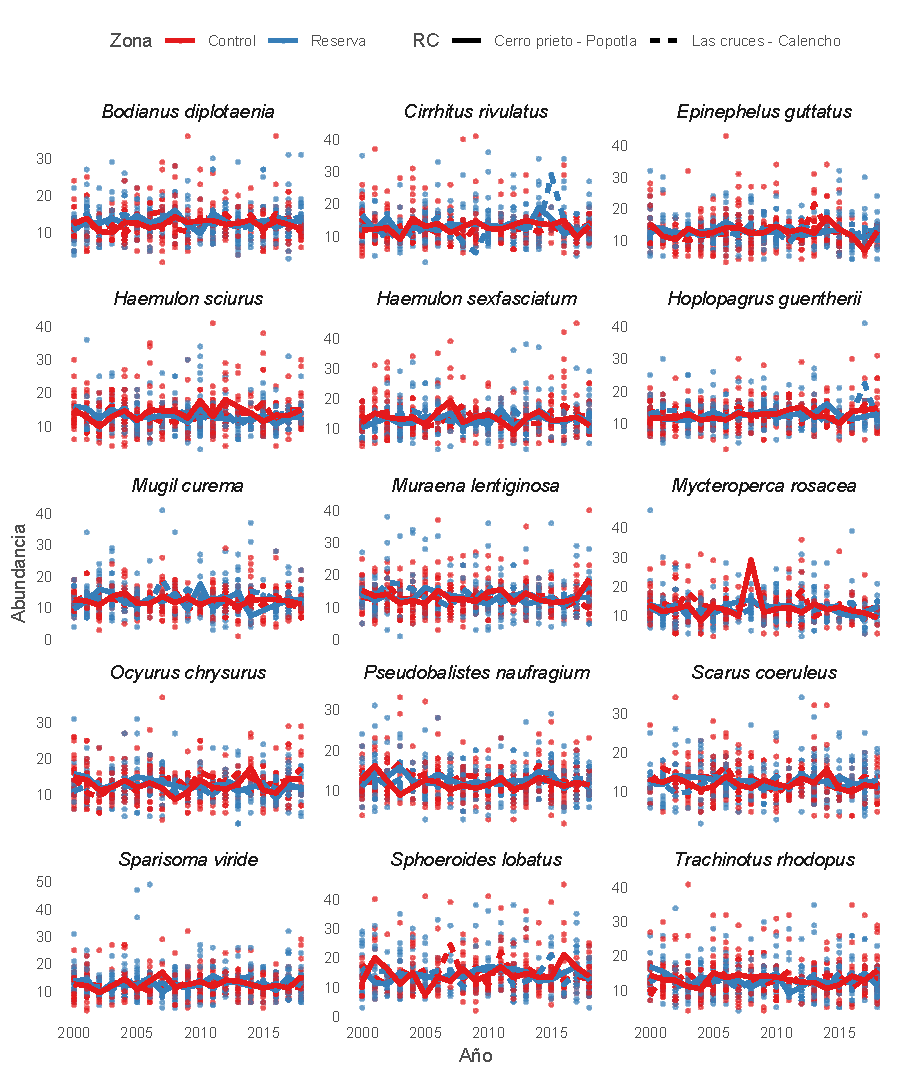
\includegraphics{evaluacion-reservas_files/figure-latex/graficar-datos-1.pdf}
\caption{\label{fig:graficar-datos}Series de tiempo de los datos antes de
agregar tendencias}
\end{figure}

\begin{Shaded}
\begin{Highlighting}[]
\CommentTok{# Ahora agregamos tendencias en abundancias y tallas.}
\CommentTok{# Las abundancias aumentan un 10% cada ano despues del 2000.}
\CommentTok{# Las tallas aumentan 1 cm cada año.}
\NormalTok{datos <-}\StringTok{ }\NormalTok{datos }\OperatorTok
\StringTok{  }\KeywordTok{mutate}\NormalTok{(}\DataTypeTok{neg =} \KeywordTok{ifelse}\NormalTok{(RC }\OperatorTok{==}\StringTok{ "Cerro prieto - Popotla"}\NormalTok{, }\DecValTok{-1}\NormalTok{, }\DecValTok{1}\NormalTok{),}
         \DataTypeTok{Abundancia =} \KeywordTok{ifelse}\NormalTok{(Zona }\OperatorTok{==}\StringTok{ "Reserva"} \OperatorTok{&}\StringTok{ }\NormalTok{Ano }\OperatorTok{>}\StringTok{ }\DecValTok{2000}\NormalTok{,}
\NormalTok{                             Abundancia }\OperatorTok{*}\StringTok{ }\NormalTok{(}\DecValTok{1} \OperatorTok{+}\StringTok{ }\NormalTok{(neg }\OperatorTok{*}\StringTok{ }\NormalTok{((Ano }\OperatorTok{-}\StringTok{ }\DecValTok{2000}\NormalTok{) }\OperatorTok{*}\StringTok{ }\FloatTok{0.1}\NormalTok{))),}
\NormalTok{                             Abundancia),}
         \DataTypeTok{Talla =} \KeywordTok{ifelse}\NormalTok{(Zona }\OperatorTok{==}\StringTok{ "Reserva"} \OperatorTok{&}\StringTok{ }\NormalTok{Ano }\OperatorTok{>}\StringTok{ }\DecValTok{2000}\NormalTok{,}
\NormalTok{                        Talla }\OperatorTok{+}\StringTok{ }\NormalTok{(neg }\OperatorTok{*}\StringTok{ }\NormalTok{((Ano }\OperatorTok{-}\StringTok{ }\DecValTok{2000}\NormalTok{) }\OperatorTok{*}\StringTok{ }\DecValTok{1}\NormalTok{)),}
\NormalTok{                        Talla)) }\OperatorTok\StringTok{ }
\StringTok{  }\KeywordTok{select}\NormalTok{(}\OperatorTok{-}\NormalTok{neg)}
\end{Highlighting}
\end{Shaded}

\begin{Shaded}
\begin{Highlighting}[]
\CommentTok{# Graficar los datos}
\KeywordTok{ggplot}\NormalTok{(}\DataTypeTok{data =}\NormalTok{ datos,}
       \DataTypeTok{mapping =} \KeywordTok{aes}\NormalTok{(}\DataTypeTok{x =}\NormalTok{ Ano, }\DataTypeTok{y =}\NormalTok{ Abundancia,}
                     \DataTypeTok{color =}\NormalTok{ Zona, }\DataTypeTok{group =}\NormalTok{ Sitio, }\DataTypeTok{linetype =}\NormalTok{ RC)) }\OperatorTok{+}
\StringTok{  }\KeywordTok{geom_point}\NormalTok{(}\DataTypeTok{alpha =} \FloatTok{0.5}\NormalTok{, }\DataTypeTok{size =} \FloatTok{0.5}\NormalTok{) }\OperatorTok{+}
\StringTok{  }\KeywordTok{stat_summary}\NormalTok{(}\DataTypeTok{geom =} \StringTok{"line"}\NormalTok{, }\DataTypeTok{fun.y =} \StringTok{"mean"}\NormalTok{, }\DataTypeTok{size =} \DecValTok{1}\NormalTok{) }\OperatorTok{+}
\StringTok{  }\KeywordTok{facet_wrap}\NormalTok{(}\OperatorTok{~}\NormalTok{GeneroEspecie, }\DataTypeTok{ncol =} \DecValTok{3}\NormalTok{, }\DataTypeTok{scales =} \StringTok{"free_y"}\NormalTok{) }\OperatorTok{+}
\StringTok{  }\NormalTok{startR}\OperatorTok{::}\KeywordTok{ggtheme_plot}\NormalTok{() }\OperatorTok{+}
\StringTok{  }\KeywordTok{theme}\NormalTok{(}\DataTypeTok{legend.position =} \StringTok{"top"}\NormalTok{) }\OperatorTok{+}
\StringTok{  }\KeywordTok{scale_color_brewer}\NormalTok{(}\DataTypeTok{palette =} \StringTok{"Set1"}\NormalTok{) }\OperatorTok{+}
\StringTok{  }\KeywordTok{xlab}\NormalTok{(}\StringTok{"Año"}\NormalTok{)}
\end{Highlighting}
\end{Shaded}

\begin{figure}
\centering
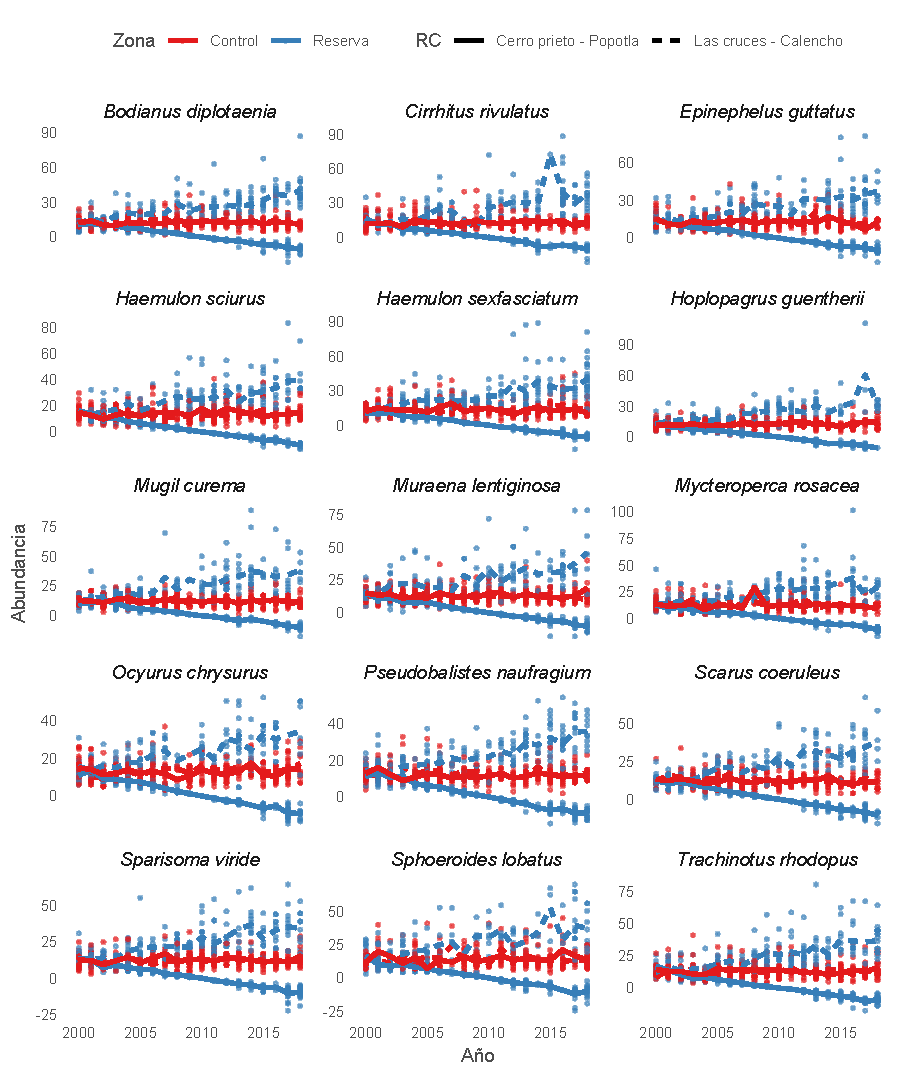
\includegraphics{evaluacion-reservas_files/figure-latex/graficar-datos-abundancias-1.pdf}
\caption{\label{fig:graficar-datos-abundancias}Series de tiempo de las
abundancias con tendencias (10\% anual) despés del primer año. Note como
una reserva funciona y otra no.}
\end{figure}

\begin{Shaded}
\begin{Highlighting}[]
\CommentTok{# Graficar los datos}
\KeywordTok{ggplot}\NormalTok{(}\DataTypeTok{data =}\NormalTok{ datos,}
       \DataTypeTok{mapping =} \KeywordTok{aes}\NormalTok{(}\DataTypeTok{x =}\NormalTok{ Ano, }\DataTypeTok{y =}\NormalTok{ Abundancia,}
                     \DataTypeTok{color =}\NormalTok{ Zona, }\DataTypeTok{group =}\NormalTok{ Sitio, }\DataTypeTok{linetype =}\NormalTok{ RC)) }\OperatorTok{+}
\StringTok{  }\KeywordTok{geom_point}\NormalTok{(}\DataTypeTok{alpha =} \FloatTok{0.5}\NormalTok{, }\DataTypeTok{size =} \FloatTok{0.5}\NormalTok{) }\OperatorTok{+}
\StringTok{  }\KeywordTok{stat_summary}\NormalTok{(}\DataTypeTok{geom =} \StringTok{"line"}\NormalTok{, }\DataTypeTok{fun.y =} \StringTok{"mean"}\NormalTok{, }\DataTypeTok{size =} \DecValTok{1}\NormalTok{) }\OperatorTok{+}
\StringTok{  }\KeywordTok{facet_wrap}\NormalTok{(}\OperatorTok{~}\NormalTok{GeneroEspecie, }\DataTypeTok{ncol =} \DecValTok{3}\NormalTok{, }\DataTypeTok{scales =} \StringTok{"free_y"}\NormalTok{) }\OperatorTok{+}
\StringTok{  }\NormalTok{startR}\OperatorTok{::}\KeywordTok{ggtheme_plot}\NormalTok{() }\OperatorTok{+}
\StringTok{  }\KeywordTok{theme}\NormalTok{(}\DataTypeTok{legend.position =} \StringTok{"top"}\NormalTok{) }\OperatorTok{+}
\StringTok{  }\KeywordTok{scale_color_brewer}\NormalTok{(}\DataTypeTok{palette =} \StringTok{"Set1"}\NormalTok{) }\OperatorTok{+}
\StringTok{  }\KeywordTok{xlab}\NormalTok{(}\StringTok{"Año"}\NormalTok{)}
\end{Highlighting}
\end{Shaded}

\begin{figure}
\centering
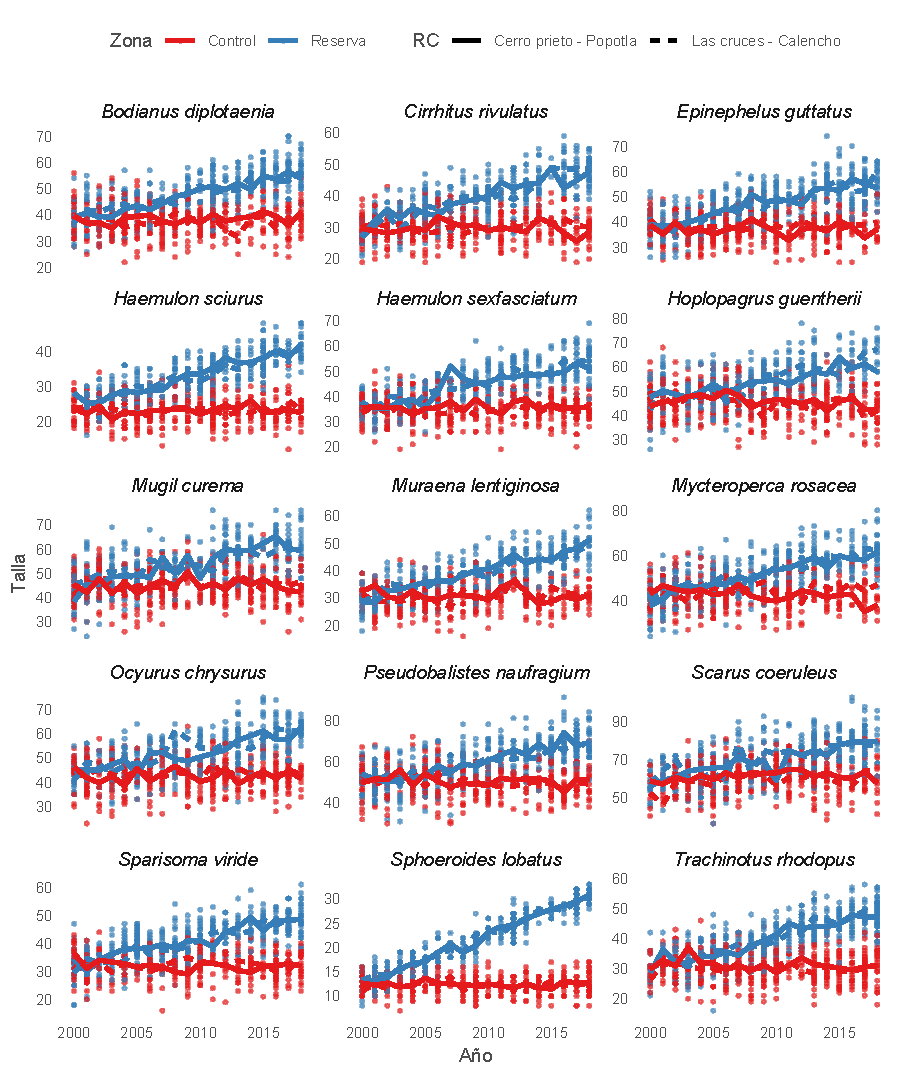
\includegraphics{evaluacion-reservas_files/figure-latex/graficar-datos-tallas-1.pdf}
\caption{\label{fig:graficar-datos-tallas}Series de tiempo de las tallas con
tendencias (+2 cm anual) despés del primer año. Note como una reserva
funciona y otra no.}
\end{figure}

\begin{Shaded}
\begin{Highlighting}[]
\KeywordTok{write.csv}\NormalTok{(}\DataTypeTok{x =}\NormalTok{ datos,}
          \DataTypeTok{file =}\NormalTok{ here}\OperatorTok{::}\KeywordTok{here}\NormalTok{(}\StringTok{"materiales"}\NormalTok{, }\StringTok{"datos"}\NormalTok{, }\StringTok{"datos_peces.csv"}\NormalTok{),}
          \DataTypeTok{row.names =}\NormalTok{ F)}
\end{Highlighting}
\end{Shaded}

\begin{Shaded}
\begin{Highlighting}[]
\CommentTok{# Generar datos para comparación de todas las reservas y todos los controles.}
\NormalTok{datos_rc <-}\StringTok{ }\NormalTok{datos }\OperatorTok\StringTok{ }
\StringTok{  }\KeywordTok{mutate}\NormalTok{(}\DataTypeTok{RC =} \StringTok{"Reserva - Control"}\NormalTok{)}
\end{Highlighting}
\end{Shaded}

\begin{Shaded}
\begin{Highlighting}[]
\KeywordTok{write.csv}\NormalTok{(}\DataTypeTok{x =}\NormalTok{ datos_rc,}
          \DataTypeTok{file =}\NormalTok{ here}\OperatorTok{::}\KeywordTok{here}\NormalTok{(}\StringTok{"materiales"}\NormalTok{, }\StringTok{"datos"}\NormalTok{, }\StringTok{"datos_peces_rc.csv"}\NormalTok{),}
          \DataTypeTok{row.names =}\NormalTok{ F)}
\end{Highlighting}
\end{Shaded}

\bibliography{references.bib,packages.bib}

\backmatter
\printindex

\end{document}
